\documentclass[conference,a4paper]{IEEEtran}
\usepackage[utf8]{inputenc}
\usepackage[T1]{fontenc}
\usepackage{textcomp}
\usepackage{graphicx}
\usepackage{booktabs}
\usepackage{amsmath}
\usepackage{url}
\usepackage{array}
\newcommand{\degC}{\,\textdegree{}C}
\newcommand{\code}[1]{\texttt{#1}}

\begin{document}

\title{Effect of Job Ordering on Thermal Throttling and Tail Latency on a Raspberry Pi~4: A Preregistered Negative Result}

% Review copy: pdflatex -jobname=paper_review "\def\REVIEW{1}\documentclass[conference,a4paper]{IEEEtran}
\usepackage[utf8]{inputenc}
\usepackage[T1]{fontenc}
\usepackage{textcomp}
\usepackage{graphicx}
\usepackage{booktabs}
\usepackage{amsmath}
\usepackage{url}
\usepackage{array}
\newcommand{\degC}{\,\textdegree{}C}
\newcommand{\code}[1]{\texttt{#1}}

\begin{document}

\title{Effect of Job Ordering on Thermal Throttling and Tail Latency on a Raspberry Pi~4: A Preregistered Negative Result}

% Review copy: pdflatex -jobname=paper_review "\def\REVIEW{1}\documentclass[conference,a4paper]{IEEEtran}
\usepackage[utf8]{inputenc}
\usepackage[T1]{fontenc}
\usepackage{textcomp}
\usepackage{graphicx}
\usepackage{booktabs}
\usepackage{amsmath}
\usepackage{url}
\usepackage{array}
\newcommand{\degC}{\,\textdegree{}C}
\newcommand{\code}[1]{\texttt{#1}}

\begin{document}

\title{Effect of Job Ordering on Thermal Throttling and Tail Latency on a Raspberry Pi~4: A Preregistered Negative Result}

% Review copy: pdflatex -jobname=paper_review "\def\REVIEW{1}\documentclass[conference,a4paper]{IEEEtran}
\usepackage[utf8]{inputenc}
\usepackage[T1]{fontenc}
\usepackage{textcomp}
\usepackage{graphicx}
\usepackage{booktabs}
\usepackage{amsmath}
\usepackage{url}
\usepackage{array}
\newcommand{\degC}{\,\textdegree{}C}
\newcommand{\code}[1]{\texttt{#1}}

\begin{document}

\title{Effect of Job Ordering on Thermal Throttling and Tail Latency on a Raspberry Pi~4: A Preregistered Negative Result}

% Review copy: pdflatex -jobname=paper_review "\def\REVIEW{1}\input{paper.tex}"
\ifdefined\REVIEW
\author{\IEEEauthorblockN{Anonymous Authors}
\IEEEauthorblockA{Names and affiliations withheld for double-blind review}}
\else
\author{\IEEEauthorblockN{Srijan Srivastava}
\IEEEauthorblockA{\textit{School of Computer Science and Engineering (SCOPE)}\\
\textit{Vellore Institute of Technology}\\
Vellore, India\\
\texttt{srijan.srivastava2023@vitstudent.ac.in}}
\and
\IEEEauthorblockN{Padma Priya}
\IEEEauthorblockA{\textit{School of Computer Science and Engineering (SCOPE)}\\
\textit{Vellore Institute of Technology}\\
Vellore, India\\
\texttt{padmapriya.r@vit.ac.in}}}
\fi

\maketitle

\begin{abstract}
On passively cooled edge devices, firmware throttles the CPU clock once the die is hot. One idea is to order
work so that heat-producing jobs are interleaved with lighter ones and fewer jobs run throttled. We tested whether
ordering alone changes tail latency. We used a Raspberry Pi~4 Model~B and a matched pair of fixed-work four-core
jobs, HOT (CPU duty 0.99) and COOL (0.38), whose cold latencies differ by $-0.05$\,\% (95\,\% CI
[$-0.08$, $-0.001$]\,\%). We compared four orderings of an identical 600-job multiset (hot-first, cool-first,
alternating, random), with 10 interleaved, counterbalanced repetitions each: 40 sequences and 24{,}000 jobs. Each
sequence started at 77.4--77.9\degC{} after a standardised cooldown and pre-heat. The hypotheses, gates and
analysis were preregistered. A throttle knee was found at 80.8\degC{} in the firmware ARM clock. Service time
rose with temperature (+0.208\,ms/\textdegree{}C, 95\,\% CI [+0.070, +0.343]): flat at about 196.4\,ms below the
knee and 208--212\,ms on the throttling plateau. Ordering changed the thermal trajectory: hot-first spent a median
13.3\,s above the knee per sequence, against 0\,s for alternating and random (difference 13.3\,s, CI [6.0, 23.8]).
It did not change tail latency: median per-sequence P99 ranged from 201.3 to 202.1\,ms across orderings, and no
pairwise difference survived Holm correction. Mean latency and throughput showed no supported difference either.
The preregistered verdict is LIKELY KILL. Exploratory analyses suggest why: throttling at this horizon is shallow,
and only about 2--3 of 600 jobs per sequence exceeded 205\,ms, so P99 is set by ordinary jobs. The device's
thermal state also shifted during the session. We report the negative result, its limits and the hypotheses it
leaves open.
\end{abstract}

\begin{IEEEkeywords}
thermal throttling, task ordering, tail latency, edge computing, Raspberry Pi, negative result, preregistration
\end{IEEEkeywords}

\section{Purpose and Objectives}
\subsection{Motivation}
Edge devices increasingly run sustained compute without active cooling. When their system-on-chip (SoC) heats up,
firmware lowers the CPU clock to stay within a thermal limit. On the Raspberry Pi~4, the vendor documents
progressive throttling of the Arm cores between 80 and 85\degC{}~\cite{rpi-thermal}. Thermal throttling has long
been studied as dynamic thermal management (DTM)~\cite{brooks2001,skadron2003}. Operating-system schedulers can
reduce thermal emergencies by choosing what runs when~\cite{choi2007,yang2008,coskun2008}. Order matters
physically: for a fixed set of tasks, the temperature reached depends on execution order~\cite{chrobak2008}.

Changing a device's thermal trajectory does not by itself change what an application observes. A throttled job is
slower only by the clock reduction it actually experiences, and a tail percentile moves only if enough jobs are
slowed by enough. A reordering that keeps the die below its knee for longer is therefore a \emph{candidate}
mechanism for lower tail latency, not evidence of it.

\subsection{Research question and objectives}
For an identical multiset of fixed-work jobs with matched cold latency, does the order
in which the jobs run change (a)~the time the device spends above its throttling knee, and (b)~the tail latency,
mean latency and throughput of the jobs?

We answer this with a preregistered, gate-based pilot on a Raspberry Pi~4, designed to falsify the idea cheaply.
Each gate's test and the verdict were fixed before the data that decided them. Every design change was recorded
as a dated amendment before the data it governed.

\textbf{Contributions} (limited to what the evidence shows):
\begin{enumerate}
\item A measured throttling knee (80.8\degC{}, firmware ARM clock) and service-time curve for this device and
workload. The Linux \code{scaling\_cur\_freq} interface did not show the throttling at all. Service time is flat
below the knee and steps up about 6--8\,\% on the throttling plateau (Sec.~\ref{sec:g1}, \ref{sec:g2}).
\item A preregistered ordering experiment with a negative primary outcome. Ordering changed the time above the
knee but produced no statistically supported change in P99, P95, mean latency or throughput at the tested
operating point. The verdict is LIKELY KILL (Sec.~\ref{sec:results}).
\item An exploratory analysis, kept separate from the confirmatory results, of why the thermal effect did not
reach the measured tail: shallow throttling at a two-minute horizon, the order statistic that a 600-job P99
measures, and a within-session shift of thermal state (Sec.~\ref{sec:discussion}--\ref{sec:claims}).
\item Disclosure of the measurement pitfalls met: an instrument blind spot, supervision that perturbed latency, and
a flawed early validity rule (Sec.~\ref{sec:integrity}).
\end{enumerate}
We propose no new scheduling algorithm and do not claim that ordering never matters. We tested one operating point
and found no supported performance effect there.

\subsection{Background and related work}
\textbf{Dynamic thermal management.} Brooks and Martonosi~\cite{brooks2001} studied DTM mechanisms that respond
when a processor nears its thermal limit. They argued that designing for typical rather than worst-case power is
possible with little performance loss. Skadron et al.~\cite{skadron2003} introduced the HotSpot model and runtime
techniques such as frequency scaling and migration. They noted that activity metrics are poor temperature proxies
and that sensor inaccuracy affects DTM. Our device uses firmware-controlled frequency reduction. The application
has no DVFS authority, which leaves ordering as one of the few levers available to software.

\textbf{Thermal-aware task scheduling.}
\begin{itemize}
\item Choi et al.~\cite{choi2007} exploited temporal and spatial ``heat slack'' through OS scheduling.
\item Yang et al.~\cite{yang2008} built a thermal-aware Linux job scheduler that exploits differences in thermal
behaviour among jobs. They reported 10.5--73.6\,\% fewer hardware DTM events and up to 7.6\,\% (average 4.1\,\%)
higher throughput.
\item Chrobak et al.~\cite{chrobak2008} formalised temperature-aware scheduling of unit jobs with heat
contributions.
\item Coskun et al.~\cite{coskun2008} reduced hot spots, gradients and thermal cycles on multiprocessor SoCs at
negligible performance cost.
\item On mobile devices, Sahin and Coskun~\cite{sahin2016} showed that throttling degrades QoS, and sustained
acceptable performance for up to $8\times$ longer.
\end{itemize}
These works establish that scheduling changes thermal behaviour, and on their platforms can change throughput or
QoS. Our study differs in four ways: it holds the \emph{work} fixed (matched jobs, differing only in order), it
uses \emph{tail latency} as the primary outcome, it runs on a low-cost single-board computer with firmware-only
DVFS, and it is preregistered with explicit kill criteria.

\textbf{Tail latency and its measurement.} Dean and Barroso~\cite{dean2013} explain why tail latency, not the mean,
governs the responsiveness of large services. Zhang et al.~\cite{zhang2016} show that tail measurements are
sensitive to load-testing methodology, and attribute tail sources by quantile regression. Sample percentiles have
several definitions~\cite{hyndman1996}; with 600 observations, a P99 rests on a handful of order statistics
(Sec.~\ref{sec:p99}). We use bootstrap intervals~\cite{efron1979}, Holm's correction~\cite{holm1979} and Cliff's
$\delta$~\cite{cliff1993}.

\textbf{Rigour and preregistration.} Hoefler and Belli~\cite{hoefler2015} give guidelines for reporting performance
results with appropriate statistics and confidence intervals. Mytkowicz et al.~\cite{mytkowicz2009} show how
innocuous setup changes bias measurements. Nosek et al.~\cite{nosek2018} argue for preregistration, which separates
confirmatory from exploratory analysis. We keep that separation throughout.

\textbf{Raspberry Pi thermal behaviour.} The official documentation describes the 80--85\degC{} throttling
range~\cite{rpi-thermal} and the \code{get\_throttled} status bits~\cite{rpi-throttled} that we use to detect
under-voltage and throttling. We found only informal vendor and hobbyist characterisations of Pi~4 cooling, not a
peer-reviewed study of job ordering against tail latency on this platform. Our search was limited, so this is not
a claim that none exists.

\section{Methodology and Approach}
\subsection{Hardware and software}
\begin{itemize}
\item \textbf{Device:} Raspberry Pi~4 Model~B Rev~1.4 (BCM2711, four Arm cores, \code{arm\_freq} 1800\,MHz,
1.8\,GiB usable memory).
\item \textbf{Software stack:} Debian~13; kernel 6.18.50+rpt-rpi-v8; firmware a8698392 (14 Sep 2026); governor
\code{performance} on all cores; no \code{temp\_limit} or \code{temp\_soft\_limit} override.
\item \textbf{Python:} 3.13.5 with NumPy 2.2.4 on the single-threaded Debian reference BLAS.
\item \textbf{Cooling:} a bare board with no heatsink or fan, in open air, as the protocol specifies. No
cooling device is registered with the kernel. The experimenter confirmed this configuration after the study; it
was not logged separately on the Experiment~3 day. Ambient temperature was not measured (Sec.~\ref{sec:limits}).
\end{itemize}

\subsection{Workload: matched fixed-work jobs}
A job uses all four cores at once: one worker per core (pinned) runs a fixed number of timed units. A unit is four
consecutive $128\times128$ single-precision matrix multiplications. Latency is measured from the dispatch of the
first shard to the reply of the last. The two job classes (frozen parameters \code{P4c-F1}) are:
\begin{itemize}
\item \textbf{HOT:} 13 units per core and no sleep (measured CPU duty 0.994).
\item \textbf{COOL:} 5 units per core with 119.55\,ms of sleep spread between them (duty 0.385).
\end{itemize}

A preregistered workload validation with 40 accepted HOT/COOL pairs accepted this pair:
\begin{itemize}
\item \textbf{Cold-latency match:} median HOT 196.32\,ms, COOL 196.22\,ms; relative gap $-0.050$\,\%, 95\,\% CI
[$-0.080$, $-0.001$]\,\%, within the preregistered $\pm2$\,\% target.
\item \textbf{Variability:} unit-time CV 0.83\,\%; HOT-latency CV 0.35\,\%.
\end{itemize}
The two classes therefore take the same time when cold but differ in heat produced. An identical multiset of them
can differ only in order. That is the manipulation: the same number of each class, the same planned units and the
same planned sleep. Energy was not measured.

\subsection{Orderings and sequences}
A sequence is 600 jobs, 300 HOT and 300 COOL, run back to back (119.6--120.4\,s). The four orderings use the
protocol's names:
\begin{itemize}
\item \code{hot\_first}: 300 HOT jobs, then 300 COOL jobs;
\item \code{cool\_first}: the reverse;
\item \code{alternating}: HOT and COOL in turn;
\item \code{random}: a new permutation for each sequence, from a seeded generator.
\end{itemize}

Each ordering was repeated 10 times. The 40 sequences were interleaved and counterbalanced: each repetition block
contains all four orderings, alternate blocks are reversed, then shuffled (seed~0).

Each sequence starts in three steps:
\begin{enumerate}
\item \textbf{Cooldown} with no load to idle\,+\,3\degC{} (48.3\degC{}), capped at 20\,min. The idle baseline,
45.28\degC{}, was measured at the start of the session.
\item \textbf{Pre-heat} with back-to-back HOT jobs, not recorded, until the temperature read before a job is at
least 77.0\degC{}. Capped at 5\,min.
\item \textbf{Sequence}, started immediately.
\end{enumerate}
Sequences started at 77.4--77.9\degC{}, just below the knee. The pre-heat took 31--53\,s.

\subsection{Measurement and supervision}
\textbf{Temperature.} SoC temperature was read from Linux sysfs (\code{thermal\_zone0}) by a 5\,Hz logger thread
during each sequence (23{,}843 samples), with readings quantised in steps of 0.487\degC{}.

\textbf{Per job.} We recorded the temperature just before dispatch, latency, CPU time and completed units. We also
recorded the firmware throttle flags (\code{vcgencmd get\_throttled}~\cite{rpi-throttled}), read between jobs and
outside the timed interval.

\textbf{What was not read live.} The firmware ARM clock was not read during Experiment~3. Live clock reads were
reserved for Experiment~2, because a stall control showed that they perturb a small fraction of jobs.

\textbf{Supervision.} An external watchdog whose loop starts no processes stops the run with a single SIGTERM at
85.0\degC{}, on under-voltage, or on failed readings. The experiment starts no load before it has verified the
watchdog. Workers are never killed with SIGKILL.

\subsection{Thermal knee}
The knee comes from a separate supervised Experiment~1 run: four HOT workers, 15\,min of continuous load, with the
cores 99.9--100\,\% busy. During it, the firmware ARM clock was read through \code{vcgencmd measure\_clock arm}. By
the preregistered definition, the knee is the lowest temperature at which the clock read below 98\,\% of the run's
maximum. Amendment A3 moved this measurement from \code{scaling\_cur\_freq} to the firmware clock before the run,
after an instrument check showed that \code{scaling\_cur\_freq} does not reflect firmware throttling on this device.

\subsection{Preregistered gates and verdict}
Table~\ref{tab:gates} lists the gates. Each was defined in the protocol or in Amendments A1--A7, before the data
it governs.

\textbf{Validity (A7).} G3--G6 are decided only by a completed, supervised session with P4c jobs, a G1 knee, and at
least 8 valid sequences per ordering. Otherwise they are INCONCLUSIVE.

\textbf{Verdict rule} (fixed before Experiment~3):
\begin{itemize}
\item a failure of a structural gate (G1, G2 or G4) is KILL;
\item G5 failing with a secondary metric responding is REFORMULATE;
\item G5 failing with no secondary response is \textbf{LIKELY KILL};
\item G1, G2, G4 and G5 all passing is PROCEED.
\end{itemize}

\begin{table*}[t]
\centering
\caption{Preregistered gates}
\label{tab:gates}
\footnotesize
\begin{tabular}{@{}l p{4.0cm} p{9.6cm} l@{}}
\toprule
Gate & Question & Test & Data\\
\midrule
G1 & Is there a throttle knee? & knee measured in a valid Exp.~1 run (A1, A3) & Exp.~1\\
G2 & Does service time depend on temperature? & OLS slope of bin-median latency on bin-median temperature; 2\degC{} bins per ramp with $\ge$20 jobs; cluster bootstrap over (ramp, bin), 2000 resamples; PASS if the 95\,\% CI $>0$ (A4) & Exp.~2\\
G3 & Are HOT and COOL indistinguishable when cold? & cold-latency gap within target in the accepted workload validation & validation\\
G4 & Does ordering change time above the knee? & largest minus smallest per-ordering median time above the knee; percentile bootstrap (10{,}000 resamples, seed 0); PASS if the 95\,\% CI excludes 0 & Exp.~3\\
G5 & Does ordering change tail latency? & 6 pairwise differences of median per-sequence P99; bootstrap $p$-values, Holm at $\alpha=0.05$ (A7); PASS if any pair survives & Exp.~3\\
G5b & Do secondary metrics respond? & the same for mean latency and throughput, Holm within each metric & Exp.~3\\
G6 & Is the effect mediated? & corr(time above knee, P99) $>0.3$, tested only if G4 and G5 pass & Exp.~3\\
\bottomrule
\end{tabular}
\end{table*}

\subsection{Statistics and unit of analysis}
\textbf{Unit of analysis.} The unit is the sequence: $n=10$ per ordering. Per-sequence P99 and P95 use NumPy's
default linear-interpolation percentile, Hyndman--Fan type~7~\cite{hyndman1996}. For 600 jobs, P99 is the
7th-largest latency, interpolated 1\,\% of the way toward the 6th largest.

\textbf{Differences.} Differences are differences of medians across sequences, with an unpaired percentile
bootstrap~\cite{efron1979}. The two-sided $p$-value is
$\min(1, 2\min(\Pr[\Delta^*\le 0], \Pr[\Delta^*\ge0]))$ over the 10{,}000 bootstrap differences~$\Delta^*$.
Effect sizes are the median difference in milliseconds and Cliff's $\delta$~\cite{cliff1993}.

\textbf{Independence.} The bootstrap treats an ordering's sequences as exchangeable. They were run serially on one
device. The interleaved, counterbalanced schedule protects the comparison from linear drift, but not from all time
dependence.

\textbf{Exploratory analyses.} Everything outside the gates is labelled exploratory and cannot change the verdict.

\subsection{Integrity checks and disclosed deviations}\label{sec:integrity}
\textbf{Integrity.} Every run archive is stored with its SHA-256 hash, which matches the copy on the device. Code on
the device was hash-pinned by the launcher. For this paper, independently written code recomputed every
per-sequence metric from the raw job and telemetry records; all matched the official record to within $10^{-6}$,
and the gate statistics and verdict reproduce exactly.

\textbf{Disclosed deviations and pitfalls:}
\begin{enumerate}
\item \textbf{Instrument blind spot.} \code{scaling\_cur\_freq} read 1800\,MHz in all 6{,}894 samples of the
Experiment~1 run, while the firmware clock fell to 1629\,MHz.
\item \textbf{Supervision perturbing the measurement.} An earlier four-core workload candidate was rejected on
latency variability. Diagnostics traced the variability to the external watchdog's process starts every 5\,s:
8~of~8 stalls fell on poll-overlapped jobs. The watchdog was rewritten to start no processes, and the accepted
configuration was validated under it.
\item \textbf{Validity-rule flaw.} The first Experiment~2 run was INCONCLUSIVE because a coverage rule could not be
met at four-core heating rates. The fix was a paced warm-up (A5), which was approved by the experimenter's
assistant under delegation and accepted by the experimenter afterwards.
\item \textbf{Safety stop.} The second Experiment~2 run was safety-stopped at 85.2\degC{}. A6 shortened each ramp.
\end{enumerate}
Both earlier Experiment~2 runs remain on record as INCONCLUSIVE, and G2 is decided by the third.

\section{Results and Findings}\label{sec:results}
\subsection{G1: throttle knee}\label{sec:g1}
In the Experiment~1 run (6{,}894 samples at 5\,Hz, no clock reading missing):
\begin{itemize}
\item The firmware ARM clock fell from 1800.5\,MHz to a minimum of 1629.4\,MHz, a depth of 9.5\,\%.
\item 477 samples were below 98\,\% of the maximum. The lowest temperature among them, the knee, was
\textbf{80.83\degC{}} (Fig.~\ref{fig:knee}), consistent with the vendor's 80--85\degC{} range~\cite{rpi-thermal}.
\item \code{scaling\_cur\_freq} never left 1800\,MHz.
\end{itemize}
G1 is \textbf{PASS}. The cooling time constant fitted in the run was 106.7\,s.

\begin{figure}[t]
\centering
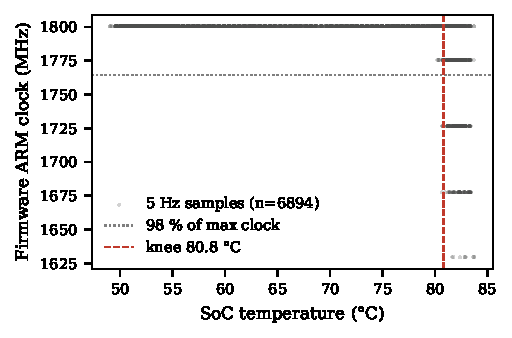
\includegraphics[width=\columnwidth]{figures/fig1_exp1_knee.pdf}
\caption{Experiment~1: firmware ARM clock against SoC temperature (6{,}894 samples at 5\,Hz, four-core load). The
knee (80.8\degC{}) is the lowest temperature at which the clock fell below 98\,\% of its maximum. Points are
jittered by $\pm0.15$\degC{} for visibility.}
\label{fig:knee}
\end{figure}

\subsection{G2: service time against temperature}\label{sec:g2}
In Experiment~2, run~3 (2 ramps, 3{,}027 HOT jobs, 36 kept bins), the OLS slope of bin-median latency on bin-median
temperature is \textbf{+0.208\,ms/\textdegree{}C} (95\,\% cluster-bootstrap CI [+0.070, +0.343]). G2 is
\textbf{PASS}.

The relationship is a step at the knee, not a line (Fig.~\ref{fig:sT}):
\begin{itemize}
\item \textbf{Below the knee:} bin medians stay within 196.23--196.55\,ms in all 30 bins, from 47.7 to 79.4\degC{}.
\item \textbf{Just above it:} 197.4--198.0\,ms at 81.3--81.8\degC{}.
\item \textbf{On the plateau:} 207.9--208.5\,ms at 83.3\degC{} and 211.0--212.1\,ms at 84.2\degC{}.
\end{itemize}

\begin{figure}[t]
\centering
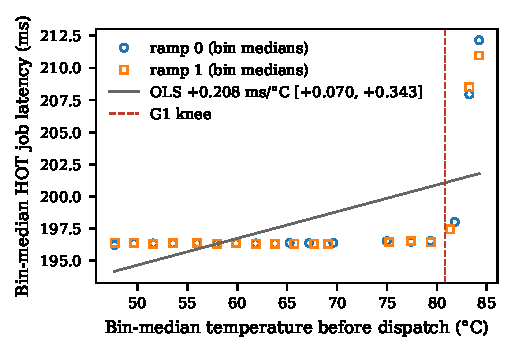
\includegraphics[width=\columnwidth]{figures/fig2_exp2_sT.pdf}
\caption{Experiment~2 (run~3): bin-median HOT job latency against bin-median temperature before dispatch (2\degC{}
bins, $\ge$20 jobs, two ramps). The preregistered OLS slope and its cluster-bootstrap CI summarise a step at the
80.8\degC{} knee.}
\label{fig:sT}
\end{figure}

\subsection{G3: cold-latency match}
In the accepted workload validation (40 pairs), median latency was 196.32\,ms for HOT and 196.22\,ms for COOL. The
gap is $-0.050$\,\% (95\,\% CI [$-0.080$, $-0.001$]\,\%), class TARGET MET. G3 is \textbf{PASS}.

\subsection{Session validity}
The Experiment~3 session ran 40 of 40 scheduled sequences in about 3\,h.
\begin{itemize}
\item All sequences were valid (10 per ordering), with no reruns.
\item No under-voltage was flagged, no watchdog signal was sent, and cleanup was verified.
\item Every sequence had exactly 300 HOT and 300 COOL jobs in its ordering's structure, and all 24{,}000 jobs
completed their planned units.
\end{itemize}
The A7 validity rule is met.

\subsection{G4: ordering and time above the knee}
Ordering changed the thermal trajectory (Fig.~\ref{fig:traj}, Fig.~\ref{fig:tak}, Table~\ref{tab:summary}):
\begin{itemize}
\item \code{hot\_first} ran up toward the knee during its HOT half.
\item \code{cool\_first} first cooled to about 61\degC{}, then climbed.
\item \code{alternating} and \code{random} settled near 71--72\degC{}.
\end{itemize}
Median time above the knee per sequence was 13.3\,s (\code{hot\_first}), 0.8\,s (\code{cool\_first}) and 0\,s
(\code{alternating}, \code{random}). The preregistered contrast between the largest and smallest median is
\textbf{+13.3\,s, 95\,\% CI [+6.0, +23.8]}. G4 is \textbf{PASS}.

\begin{figure}[t]
\centering
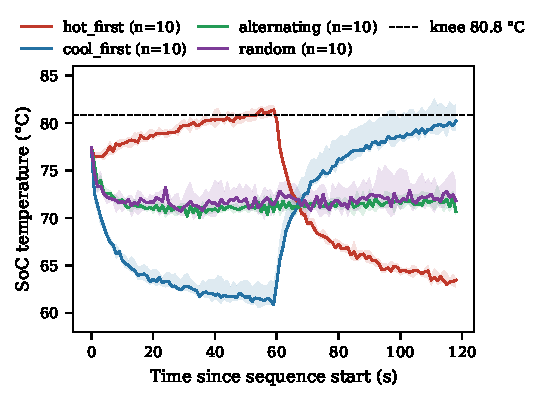
\includegraphics[width=\columnwidth]{figures/fig3_exp3_trajectories.pdf}
\caption{Experiment~3: SoC temperature during the 600-job sequences; median (line) and interquartile range (band)
across the 10 sequences of each ordering, aligned at sequence start.}
\label{fig:traj}
\end{figure}

\begin{figure}[t]
\centering
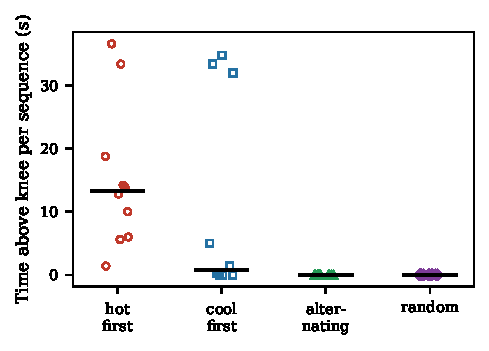
\includegraphics[width=\columnwidth]{figures/fig4_exp3_time_above_knee.pdf}
\caption{Experiment~3: time above the 80.8\degC{} knee per sequence (points) and per-ordering median (bar).}
\label{fig:tak}
\end{figure}

\begin{table*}[t]
\centering
\caption{Per-ordering summary, median [interquartile range] over 10 valid sequences each}
\label{tab:summary}
\footnotesize
\begin{tabular}{@{}lllll@{}}
\toprule
 & hot\_first & cool\_first & alternating & random\\
\midrule
Time above knee (s) & 13.3 [7.0, 17.7] & 0.8 [0.0, 25.3] & 0.0 [0.0, 0.0] & 0.0 [0.0, 0.0]\\
Peak temperature (\textdegree{}C) & 82.3 & 81.1 & 77.4 & 77.4\\
P99 latency (ms) & 201.26 [201.05, 201.61] & 201.35 [200.27, 207.60] & 202.14 [201.76, 202.42] & 201.51 [201.34, 201.83]\\
P95 latency (ms) & 199.39 & 199.44 & 199.40 & 199.34\\
Mean latency (ms) & 197.14 & 197.11 & 197.20 & 197.09\\
Throughput (jobs/s) & 5.014 & 5.015 & 5.013 & 5.015\\
\bottomrule
\end{tabular}
\end{table*}

\subsection{G5 and G5b: tail latency, mean latency, throughput}
Median per-sequence P99 differed by at most 0.88\,ms (0.44\,\%) between any two orderings (Fig.~\ref{fig:out},
Table~\ref{tab:pairs}).
\begin{itemize}
\item \textbf{Uncorrected:} one pair's CI excluded zero (\code{alternating} $-$ \code{random}, +0.62\,ms,
$p=0.046$).
\item \textbf{Holm:} with six pairs, Holm's first step needs $p\le0.0083$, so no pair survives. G5 is
\textbf{FAIL}.
\item \textbf{Secondary metrics:} for mean latency and throughput, the smallest $p$-values (0.037 and 0.045, the same
pair) also fail Holm's first step. G5b is \textbf{FAIL}.
\end{itemize}

\begin{figure*}[t]
\centering
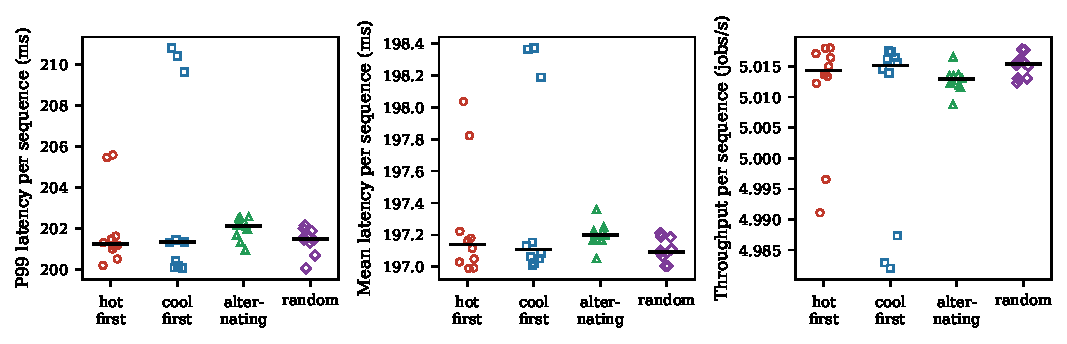
\includegraphics[width=\textwidth]{figures/fig5_exp3_outcomes.pdf}
\caption{Experiment~3: per-sequence P99 latency, mean latency and throughput by ordering (points; horizontal jitter
only), with medians (bars).}
\label{fig:out}
\end{figure*}

\begin{table}[t]
\centering
\caption{Pairwise differences in median per-sequence P99 (ms): bootstrap 95\,\% CI, two-sided bootstrap $p$, Holm
decision, Cliff's $\delta$}
\label{tab:pairs}
\footnotesize
\setlength{\tabcolsep}{3pt}
\begin{tabular}{@{}lrrrcr@{}}
\toprule
Pair & $\Delta$ & 95\,\% CI & $p$ & Holm & $\delta$\\
\midrule
alt $-$ cool & +0.79 & [$-7.66$, +1.97] & 0.306 & no & +0.30\\
alt $-$ hot & +0.88 & [$-1.29$, +1.36] & 0.068 & no & +0.44\\
alt $-$ rand & +0.62 & [+0.01, +1.08] & 0.046 & no & +0.56\\
cool $-$ hot & +0.09 & [$-1.97$, +8.45] & 0.979 & no & +0.00\\
cool $-$ rand & $-0.16$ & [$-1.39$, +8.18] & 0.389 & no & $-0.12$\\
hot $-$ rand & $-0.26$ & [$-0.75$, +1.90] & 0.340 & no & $-0.14$\\
\bottomrule
\end{tabular}
\end{table}

\subsection{G6 and verdict}
G6 is defined only if G4 and G5 both pass. Because G5 failed, G6 is \textbf{not testable}.

The committed analysis code, applied to the Experiment~1--3 records, returns G1--G4 PASS, G5 and G5b FAIL, and the
preregistered verdict \textbf{LIKELY KILL}: the thermal trajectory moves, but no performance metric responds.
Independently written code reproduces this verdict from the raw records.

\subsection{A thermal effect without a performance effect}\label{sec:discussion}
Ordering changed \emph{when} and \emph{for how long} the die was above its knee (G4). It did not move the latency
distribution enough to register in P99, mean latency or throughput (G5, G5b). The exploratory analyses below,
which cannot change the verdict, suggest why.

\textbf{At a two-minute horizon starting just below the knee, throttling is shallow.}
\begin{itemize}
\item Of 12{,}000 HOT jobs, 1{,}258 started at or above the knee. Their median latency was 198.29\,ms, against
196.87\,ms for HOT jobs below it (+0.7\,\%). Their 90th percentiles were 204.99 and 198.98\,ms.
\item The deeper clock reductions behind the 208--212\,ms plateau of Experiment~2 appear only after minutes of
continuous load. A \code{hot\_first} sequence runs at most 60\,s of HOT work.
\item In \code{hot\_first} sequences, a median 60 jobs per sequence (10\,\%) started at or above the knee, but most
of them were only slightly slower.
\end{itemize}

\subsection{What P99 measures for 600 jobs}\label{sec:p99}
Per sequence, P99 is in effect the 7th-largest of 600 latencies, and slow jobs are scarce:
\begin{itemize}
\item The median number of jobs slower than 205\,ms per sequence was 2.5, 2.5, 2.0 and 2.5 across orderings. The
number slower than 200\,ms was 14.5--18.
\item The 7th-largest latency is therefore usually an ordinary job of about 200--202\,ms, not a throttled one, in
every ordering.
\item The rare extreme outliers (11--15 jobs above 215\,ms per ordering, out of 6{,}000) mostly started below the
knee.
\item A job-level bootstrap within a sequence (assuming exchangeable jobs) gives a median 95\,\% interval width of
3.3\,ms for one sequence's P99.
\end{itemize}

\textbf{Sensitivity.} A rough normal approximation on the per-sequence P99 spread suggests that, with 10 sequences
per ordering and 80\,\% power at Holm's first step, detectable effects range from about 0.9\,ms
(\code{alternating} vs \code{random}) to 5.6\,ms (pairs involving \code{cool\_first}). The observed median
differences, $\le0.9$\,ms, are below most of these. A non-significant result is not equivalence. What the data
support is narrower: at this operating point, any ordering effect on the median per-sequence P99 is small relative
to a 196\,ms job, and the observed differences were under 0.5\,\%.

\subsection{Starting state and the session}
The preregistered design fixed a near-knee start (77\degC{}) and a two-minute horizon. Exploratory observations
show how much the outcome depends on thermal state (Fig.~\ref{fig:session}).

\textbf{Repetitions 0--2 (the first $\sim$70\,min):}
\begin{itemize}
\item Median cooldowns to 48.3\degC{} were 152, 217 and 262\,s, and median pre-heats 32--36\,s.
\item In 5 of the 6 \code{hot\_first} and \code{cool\_first} sequences, the die spent 32--37\,s above the knee, and
P99 was 205.5--210.8\,ms.
\item The \code{alternating} and \code{random} sequences of the same repetitions stayed at 200.1--202.6\,ms.
\end{itemize}

\textbf{Repetitions 3--9:} median cooldowns were 57--75\,s and median pre-heats 43--48\,s. P99 was
200.1--202.5\,ms in every ordering.

The cause is unknown; ambient temperature and airflow were not measured. Because every repetition contains all four
orderings, the shift adds variance rather than bias to the ordering comparison, and it produces the wide CIs for the
\code{cool\_first} pairs.

\textbf{A hypothesis, not a result.} When the device is loaded enough that blocked orderings spend more than about
30\,s above the knee within a sequence, ordering may move P99 by several milliseconds (2--5\,\%). That would need a
separately preregistered study with controlled ambient conditions.

\textbf{Pooling.} Pooling all 6{,}000 jobs of an ordering gives P99 values of 204.1, 207.9, 202.2 and 201.6\,ms
(Fig.~\ref{fig:ccdf}). These are dominated by the few hot early sequences. They are not the preregistered
statistic, but they show that the choice of summary changes the impression.

\begin{figure}[t]
\centering
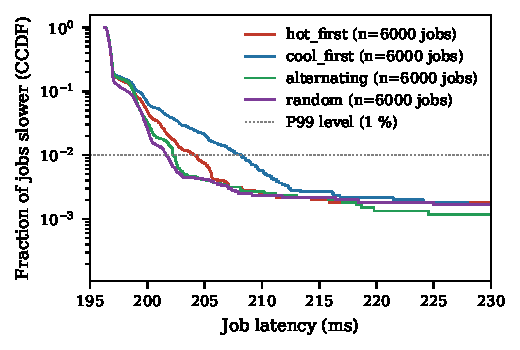
\includegraphics[width=\columnwidth]{figures/fig6_exp3_tail_ccdf_exploratory.pdf}
\caption{Exploratory: complementary CDF of job latency, all 6{,}000 jobs of each ordering (log scale). Not the
preregistered statistic; pooled tails are dominated by a few early-session sequences.}
\label{fig:ccdf}
\end{figure}

\begin{figure}[t]
\centering
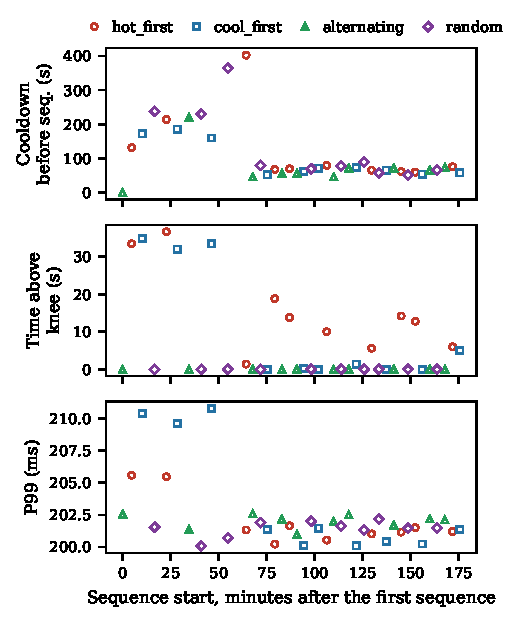
\includegraphics[width=\columnwidth]{figures/fig7_exp3_session_order_exploratory.pdf}
\caption{Exploratory: cooldown before each sequence, time above the knee, and P99 per sequence against session time.
The first $\sim$70\,min show long cooldowns and, for the blocked orderings, long times above the knee and higher
P99. (The first sequence needed no cooldown.)}
\label{fig:session}
\end{figure}

\subsection{Alternative explanations and supported claims}\label{sec:claims}
\textbf{Order effects.} Job-length differences are excluded within the validated tolerance (G3). Linear drift is
balanced by the schedule. Nonlinear drift is not excluded, but it is symmetric across orderings within each
repetition.

\textbf{Non-thermal outliers.} The extreme outliers above 215\,ms were spread evenly across orderings and mostly
started below the knee. This suggests operating-system or timing noise rather than throttling.

\textbf{Measurement perturbation.} The between-job flag reads and the 60\,s status observer were present in all
orderings alike.

\textbf{What we can and cannot conclude.}
\begin{itemize}
\item \textbf{Supported:} the causal claim that ordering changes time above the knee. The orderings were randomised
in order and the work was identical.
\item \textbf{Not supported:} the claim that ordering has \emph{no} effect on tail latency. The data allow small
effects, and larger ones in thermal states the session did not control.
\item \textbf{Physical versus practical:} the physical effect (G4) is real. A practically useful effect was not
observed.
\end{itemize}

\subsection{Limitations and threats to validity}\label{sec:limits}
\textbf{Generalisability.}
\begin{itemize}
\item One device and one environment; the bare-board configuration was confirmed afterwards, not logged on the day.
\item Ambient temperature was not measured.
\item One synthetic GEMM workload, without the memory, I/O or accelerator behaviour of real inference.
\item One sequence length (600 jobs) and one start band (77\degC{}); the protocol's sweep of three start
temperatures was not run.
\end{itemize}

\textbf{Power and percentile estimation.} Ten sequences per ordering cannot resolve sub-millisecond P99 effects.
P99 over 600 jobs rests on about 7 order statistics.

\textbf{Statistical assumptions.}
\begin{itemize}
\item The bootstrap assumes exchangeable sequences despite serial execution and a mid-session shift.
\item G4 compares a pair selected from the data, as preregistered.
\item Holm controls error within each metric only.
\end{itemize}

\textbf{Sensors.} The sensor is quantised at 0.487\degC{} and sampled at 5\,Hz. Time above the knee uses sysfs
temperature, not the firmware clock.

\textbf{Interference.} Between-job flag reads use a short-lived process, and a status observer polled every
60\,s. Both were present in all orderings.

\textbf{Process.} One amendment (A5) was approved under delegation before the experimenter reviewed it. Two Experiment~2
runs were inconclusive before G2 was decided. Both are disclosed.

\section{Conclusion and Future Scope}
On a passively cooled Raspberry Pi~4 running matched fixed-work four-core jobs, the order of an identical job
multiset changed how long the device spent above its throttling knee. At the preregistered operating point
(600-job sequences starting at 77\degC{}), that change did not produce a statistically supported difference in P99
latency, mean latency or throughput. The preregistered verdict is LIKELY KILL for the claim that ordering alone
improves tail latency on this device.

\textbf{Future scope.} The following are future experiments, not findings. Each needs its own preregistered
hypothesis, protocol and success criteria, and none can revise this verdict:
\begin{itemize}
\item longer hot blocks that reach the deep throttling plateau, within safety limits;
\item controlled initial thermal states and ambient conditions;
\item tail-sensitive designs sized by a power analysis from the variance reported here;
\item other devices, cooling configurations and real inference workloads.
\end{itemize}

\ifdefined\REVIEW\else
\section*{Author Contributions}
Srijan Srivastava carried out the research and prepared the paper. Padma Priya supervised the work and provided guidance.
\fi

\section*{Acknowledgment}
The authors used Claude (Anthropic), a generative AI assistant, throughout this work to help write and test the code, analyse the data, and draft the text and figures, and it approved amendment A5 under delegation; the authors reviewed the output and take full responsibility for the content.

\begin{thebibliography}{18}
\bibitem{brooks2001} D.~Brooks and M.~Martonosi, ``Dynamic thermal management for high-performance microprocessors,'' in \emph{Proc. 7th Int. Symp. High-Performance Computer Architecture (HPCA)}, 2001, pp. 171--182, doi: 10.1109/HPCA.2001.903261.
\bibitem{skadron2003} K.~Skadron, M.~R. Stan, W.~Huang, S.~Velusamy, K.~Sankaranarayanan, and D.~Tarjan, ``Temperature-aware microarchitecture,'' in \emph{Proc. 30th Annu. Int. Symp. Computer Architecture (ISCA)}, 2003, pp. 2--13, doi: 10.1145/859618.859620.
\bibitem{choi2007} J.~Choi, C.-Y. Cher, H.~Franke, H.~Hamann, A.~Weger, and P.~Bose, ``Thermal-aware task scheduling at the system software level,'' in \emph{Proc. Int. Symp. Low Power Electronics and Design (ISLPED)}, 2007, pp. 213--218, doi: 10.1145/1283780.1283826.
\bibitem{yang2008} J.~Yang, X.~Zhou, M.~Chrobak, Y.~Zhang, and L.~Jin, ``Dynamic thermal management through task scheduling,'' in \emph{Proc. IEEE Int. Symp. Performance Analysis of Systems and Software (ISPASS)}, 2008, pp. 191--201, doi: 10.1109/ISPASS.2008.4510751.
\bibitem{chrobak2008} M.~Chrobak, C.~D\"urr, M.~Hurand, and J.~Robert, ``Algorithms for temperature-aware task scheduling in microprocessor systems,'' in \emph{Algorithmic Aspects in Information and Management (AAIM)}, ser. Lecture Notes in Computer Science.\hskip 1em plus 0.5em minus 0.4em\relax Springer, 2008, pp. 120--130, doi: 10.1007/978-3-540-68880-8\_13.
\bibitem{coskun2008} A.~K. Coskun, T.~S. Rosing, K.~A. Whisnant, and K.~C. Gross, ``Static and dynamic temperature-aware scheduling for multiprocessor SoCs,'' \emph{IEEE Trans. Very Large Scale Integr. (VLSI) Syst.}, vol.~16, no.~9, pp. 1127--1140, 2008, doi: 10.1109/TVLSI.2008.2000726.
\bibitem{sahin2016} O.~Sahin and A.~K. Coskun, ``Providing sustainable performance in thermally constrained mobile devices,'' in \emph{Proc. 14th ACM/IEEE Symp. Embedded Systems for Real-Time Multimedia (ESTIMedia)}, 2016, pp. 72--77, doi: 10.1145/2993452.2994309.
\bibitem{rpi-thermal} Raspberry Pi Ltd, ``Raspberry Pi computer hardware: Frequency management and thermal control,'' Raspberry Pi Documentation. [Online]. Available: \url{https://www.raspberrypi.com/documentation/computers/raspberry-pi.html} (accessed Oct. 18, 2026).
\bibitem{rpi-throttled} Raspberry Pi Ltd, ``Raspberry Pi OS: vcgencmd get\_throttled,'' Raspberry Pi Documentation. [Online]. Available: \url{https://www.raspberrypi.com/documentation/computers/os.html} (accessed Oct. 18, 2026).
\bibitem{dean2013} J.~Dean and L.~A. Barroso, ``The tail at scale,'' \emph{Commun. ACM}, vol.~56, no.~2, pp. 74--80, 2013, doi: 10.1145/2408776.2408794.
\bibitem{zhang2016} Y.~Zhang, D.~Meisner, J.~Mars, and L.~Tang, ``Treadmill: Attributing the source of tail latency through precise load testing and statistical inference,'' in \emph{Proc. ACM/IEEE 43rd Annu. Int. Symp. Computer Architecture (ISCA)}, 2016, pp. 456--468, doi: 10.1109/ISCA.2016.47.
\bibitem{hyndman1996} R.~J. Hyndman and Y.~Fan, ``Sample quantiles in statistical packages,'' \emph{Amer. Statistician}, vol.~50, no.~4, pp. 361--365, 1996, doi: 10.1080/00031305.1996.10473566.
\bibitem{efron1979} B.~Efron, ``Bootstrap methods: Another look at the jackknife,'' \emph{Ann. Statist.}, vol.~7, no.~1, pp. 1--26, 1979, doi: 10.1214/aos/1176344552.
\bibitem{holm1979} S.~Holm, ``A simple sequentially rejective multiple test procedure,'' \emph{Scand. J. Statist.}, vol.~6, pp. 65--70, 1979. [Online]. Available: \url{https://www.jstor.org/stable/4615733}
\bibitem{cliff1993} N.~Cliff, ``Dominance statistics: Ordinal analyses to answer ordinal questions,'' \emph{Psychol. Bull.}, vol.~114, no.~3, pp. 494--509, 1993, doi: 10.1037/0033-2909.114.3.494.
\bibitem{hoefler2015} T.~Hoefler and R.~Belli, ``Scientific benchmarking of parallel computing systems: Twelve ways to tell the masses when reporting performance results,'' in \emph{Proc. Int. Conf. High Performance Computing, Networking, Storage and Analysis (SC)}, 2015, pp. 1--12, doi: 10.1145/2807591.2807644.
\bibitem{mytkowicz2009} T.~Mytkowicz, A.~Diwan, M.~Hauswirth, and P.~F. Sweeney, ``Producing wrong data without doing anything obviously wrong!'' in \emph{Proc. 14th Int. Conf. Architectural Support for Programming Languages and Operating Systems (ASPLOS)}, 2009, pp. 265--276, doi: 10.1145/1508244.1508275.
\bibitem{nosek2018} B.~A. Nosek, C.~R. Ebersole, A.~C. DeHaven, and D.~T. Mellor, ``The preregistration revolution,'' \emph{Proc. Natl. Acad. Sci. USA}, vol.~115, no.~11, pp. 2600--2606, 2018, doi: 10.1073/pnas.1708274114.
\end{thebibliography}

\end{document}
"
\ifdefined\REVIEW
\author{\IEEEauthorblockN{Anonymous Authors}
\IEEEauthorblockA{Names and affiliations withheld for double-blind review}}
\else
\author{\IEEEauthorblockN{Srijan Srivastava}
\IEEEauthorblockA{\textit{School of Computer Science and Engineering (SCOPE)}\\
\textit{Vellore Institute of Technology}\\
Vellore, India\\
\texttt{srijan.srivastava2023@vitstudent.ac.in}}
\and
\IEEEauthorblockN{Padma Priya}
\IEEEauthorblockA{\textit{School of Computer Science and Engineering (SCOPE)}\\
\textit{Vellore Institute of Technology}\\
Vellore, India\\
\texttt{padmapriya.r@vit.ac.in}}}
\fi

\maketitle

\begin{abstract}
On passively cooled edge devices, firmware throttles the CPU clock once the die is hot. One idea is to order
work so that heat-producing jobs are interleaved with lighter ones and fewer jobs run throttled. We tested whether
ordering alone changes tail latency. We used a Raspberry Pi~4 Model~B and a matched pair of fixed-work four-core
jobs, HOT (CPU duty 0.99) and COOL (0.38), whose cold latencies differ by $-0.05$\,\% (95\,\% CI
[$-0.08$, $-0.001$]\,\%). We compared four orderings of an identical 600-job multiset (hot-first, cool-first,
alternating, random), with 10 interleaved, counterbalanced repetitions each: 40 sequences and 24{,}000 jobs. Each
sequence started at 77.4--77.9\degC{} after a standardised cooldown and pre-heat. The hypotheses, gates and
analysis were preregistered. A throttle knee was found at 80.8\degC{} in the firmware ARM clock. Service time
rose with temperature (+0.208\,ms/\textdegree{}C, 95\,\% CI [+0.070, +0.343]): flat at about 196.4\,ms below the
knee and 208--212\,ms on the throttling plateau. Ordering changed the thermal trajectory: hot-first spent a median
13.3\,s above the knee per sequence, against 0\,s for alternating and random (difference 13.3\,s, CI [6.0, 23.8]).
It did not change tail latency: median per-sequence P99 ranged from 201.3 to 202.1\,ms across orderings, and no
pairwise difference survived Holm correction. Mean latency and throughput showed no supported difference either.
The preregistered verdict is LIKELY KILL. Exploratory analyses suggest why: throttling at this horizon is shallow,
and only about 2--3 of 600 jobs per sequence exceeded 205\,ms, so P99 is set by ordinary jobs. The device's
thermal state also shifted during the session. We report the negative result, its limits and the hypotheses it
leaves open.
\end{abstract}

\begin{IEEEkeywords}
thermal throttling, task ordering, tail latency, edge computing, Raspberry Pi, negative result, preregistration
\end{IEEEkeywords}

\section{Purpose and Objectives}
\subsection{Motivation}
Edge devices increasingly run sustained compute without active cooling. When their system-on-chip (SoC) heats up,
firmware lowers the CPU clock to stay within a thermal limit. On the Raspberry Pi~4, the vendor documents
progressive throttling of the Arm cores between 80 and 85\degC{}~\cite{rpi-thermal}. Thermal throttling has long
been studied as dynamic thermal management (DTM)~\cite{brooks2001,skadron2003}. Operating-system schedulers can
reduce thermal emergencies by choosing what runs when~\cite{choi2007,yang2008,coskun2008}. Order matters
physically: for a fixed set of tasks, the temperature reached depends on execution order~\cite{chrobak2008}.

Changing a device's thermal trajectory does not by itself change what an application observes. A throttled job is
slower only by the clock reduction it actually experiences, and a tail percentile moves only if enough jobs are
slowed by enough. A reordering that keeps the die below its knee for longer is therefore a \emph{candidate}
mechanism for lower tail latency, not evidence of it.

\subsection{Research question and objectives}
For an identical multiset of fixed-work jobs with matched cold latency, does the order
in which the jobs run change (a)~the time the device spends above its throttling knee, and (b)~the tail latency,
mean latency and throughput of the jobs?

We answer this with a preregistered, gate-based pilot on a Raspberry Pi~4, designed to falsify the idea cheaply.
Each gate's test and the verdict were fixed before the data that decided them. Every design change was recorded
as a dated amendment before the data it governed.

\textbf{Contributions} (limited to what the evidence shows):
\begin{enumerate}
\item A measured throttling knee (80.8\degC{}, firmware ARM clock) and service-time curve for this device and
workload. The Linux \code{scaling\_cur\_freq} interface did not show the throttling at all. Service time is flat
below the knee and steps up about 6--8\,\% on the throttling plateau (Sec.~\ref{sec:g1}, \ref{sec:g2}).
\item A preregistered ordering experiment with a negative primary outcome. Ordering changed the time above the
knee but produced no statistically supported change in P99, P95, mean latency or throughput at the tested
operating point. The verdict is LIKELY KILL (Sec.~\ref{sec:results}).
\item An exploratory analysis, kept separate from the confirmatory results, of why the thermal effect did not
reach the measured tail: shallow throttling at a two-minute horizon, the order statistic that a 600-job P99
measures, and a within-session shift of thermal state (Sec.~\ref{sec:discussion}--\ref{sec:claims}).
\item Disclosure of the measurement pitfalls met: an instrument blind spot, supervision that perturbed latency, and
a flawed early validity rule (Sec.~\ref{sec:integrity}).
\end{enumerate}
We propose no new scheduling algorithm and do not claim that ordering never matters. We tested one operating point
and found no supported performance effect there.

\subsection{Background and related work}
\textbf{Dynamic thermal management.} Brooks and Martonosi~\cite{brooks2001} studied DTM mechanisms that respond
when a processor nears its thermal limit. They argued that designing for typical rather than worst-case power is
possible with little performance loss. Skadron et al.~\cite{skadron2003} introduced the HotSpot model and runtime
techniques such as frequency scaling and migration. They noted that activity metrics are poor temperature proxies
and that sensor inaccuracy affects DTM. Our device uses firmware-controlled frequency reduction. The application
has no DVFS authority, which leaves ordering as one of the few levers available to software.

\textbf{Thermal-aware task scheduling.}
\begin{itemize}
\item Choi et al.~\cite{choi2007} exploited temporal and spatial ``heat slack'' through OS scheduling.
\item Yang et al.~\cite{yang2008} built a thermal-aware Linux job scheduler that exploits differences in thermal
behaviour among jobs. They reported 10.5--73.6\,\% fewer hardware DTM events and up to 7.6\,\% (average 4.1\,\%)
higher throughput.
\item Chrobak et al.~\cite{chrobak2008} formalised temperature-aware scheduling of unit jobs with heat
contributions.
\item Coskun et al.~\cite{coskun2008} reduced hot spots, gradients and thermal cycles on multiprocessor SoCs at
negligible performance cost.
\item On mobile devices, Sahin and Coskun~\cite{sahin2016} showed that throttling degrades QoS, and sustained
acceptable performance for up to $8\times$ longer.
\end{itemize}
These works establish that scheduling changes thermal behaviour, and on their platforms can change throughput or
QoS. Our study differs in four ways: it holds the \emph{work} fixed (matched jobs, differing only in order), it
uses \emph{tail latency} as the primary outcome, it runs on a low-cost single-board computer with firmware-only
DVFS, and it is preregistered with explicit kill criteria.

\textbf{Tail latency and its measurement.} Dean and Barroso~\cite{dean2013} explain why tail latency, not the mean,
governs the responsiveness of large services. Zhang et al.~\cite{zhang2016} show that tail measurements are
sensitive to load-testing methodology, and attribute tail sources by quantile regression. Sample percentiles have
several definitions~\cite{hyndman1996}; with 600 observations, a P99 rests on a handful of order statistics
(Sec.~\ref{sec:p99}). We use bootstrap intervals~\cite{efron1979}, Holm's correction~\cite{holm1979} and Cliff's
$\delta$~\cite{cliff1993}.

\textbf{Rigour and preregistration.} Hoefler and Belli~\cite{hoefler2015} give guidelines for reporting performance
results with appropriate statistics and confidence intervals. Mytkowicz et al.~\cite{mytkowicz2009} show how
innocuous setup changes bias measurements. Nosek et al.~\cite{nosek2018} argue for preregistration, which separates
confirmatory from exploratory analysis. We keep that separation throughout.

\textbf{Raspberry Pi thermal behaviour.} The official documentation describes the 80--85\degC{} throttling
range~\cite{rpi-thermal} and the \code{get\_throttled} status bits~\cite{rpi-throttled} that we use to detect
under-voltage and throttling. We found only informal vendor and hobbyist characterisations of Pi~4 cooling, not a
peer-reviewed study of job ordering against tail latency on this platform. Our search was limited, so this is not
a claim that none exists.

\section{Methodology and Approach}
\subsection{Hardware and software}
\begin{itemize}
\item \textbf{Device:} Raspberry Pi~4 Model~B Rev~1.4 (BCM2711, four Arm cores, \code{arm\_freq} 1800\,MHz,
1.8\,GiB usable memory).
\item \textbf{Software stack:} Debian~13; kernel 6.18.50+rpt-rpi-v8; firmware a8698392 (14 Sep 2026); governor
\code{performance} on all cores; no \code{temp\_limit} or \code{temp\_soft\_limit} override.
\item \textbf{Python:} 3.13.5 with NumPy 2.2.4 on the single-threaded Debian reference BLAS.
\item \textbf{Cooling:} a bare board with no heatsink or fan, in open air, as the protocol specifies. No
cooling device is registered with the kernel. The experimenter confirmed this configuration after the study; it
was not logged separately on the Experiment~3 day. Ambient temperature was not measured (Sec.~\ref{sec:limits}).
\end{itemize}

\subsection{Workload: matched fixed-work jobs}
A job uses all four cores at once: one worker per core (pinned) runs a fixed number of timed units. A unit is four
consecutive $128\times128$ single-precision matrix multiplications. Latency is measured from the dispatch of the
first shard to the reply of the last. The two job classes (frozen parameters \code{P4c-F1}) are:
\begin{itemize}
\item \textbf{HOT:} 13 units per core and no sleep (measured CPU duty 0.994).
\item \textbf{COOL:} 5 units per core with 119.55\,ms of sleep spread between them (duty 0.385).
\end{itemize}

A preregistered workload validation with 40 accepted HOT/COOL pairs accepted this pair:
\begin{itemize}
\item \textbf{Cold-latency match:} median HOT 196.32\,ms, COOL 196.22\,ms; relative gap $-0.050$\,\%, 95\,\% CI
[$-0.080$, $-0.001$]\,\%, within the preregistered $\pm2$\,\% target.
\item \textbf{Variability:} unit-time CV 0.83\,\%; HOT-latency CV 0.35\,\%.
\end{itemize}
The two classes therefore take the same time when cold but differ in heat produced. An identical multiset of them
can differ only in order. That is the manipulation: the same number of each class, the same planned units and the
same planned sleep. Energy was not measured.

\subsection{Orderings and sequences}
A sequence is 600 jobs, 300 HOT and 300 COOL, run back to back (119.6--120.4\,s). The four orderings use the
protocol's names:
\begin{itemize}
\item \code{hot\_first}: 300 HOT jobs, then 300 COOL jobs;
\item \code{cool\_first}: the reverse;
\item \code{alternating}: HOT and COOL in turn;
\item \code{random}: a new permutation for each sequence, from a seeded generator.
\end{itemize}

Each ordering was repeated 10 times. The 40 sequences were interleaved and counterbalanced: each repetition block
contains all four orderings, alternate blocks are reversed, then shuffled (seed~0).

Each sequence starts in three steps:
\begin{enumerate}
\item \textbf{Cooldown} with no load to idle\,+\,3\degC{} (48.3\degC{}), capped at 20\,min. The idle baseline,
45.28\degC{}, was measured at the start of the session.
\item \textbf{Pre-heat} with back-to-back HOT jobs, not recorded, until the temperature read before a job is at
least 77.0\degC{}. Capped at 5\,min.
\item \textbf{Sequence}, started immediately.
\end{enumerate}
Sequences started at 77.4--77.9\degC{}, just below the knee. The pre-heat took 31--53\,s.

\subsection{Measurement and supervision}
\textbf{Temperature.} SoC temperature was read from Linux sysfs (\code{thermal\_zone0}) by a 5\,Hz logger thread
during each sequence (23{,}843 samples), with readings quantised in steps of 0.487\degC{}.

\textbf{Per job.} We recorded the temperature just before dispatch, latency, CPU time and completed units. We also
recorded the firmware throttle flags (\code{vcgencmd get\_throttled}~\cite{rpi-throttled}), read between jobs and
outside the timed interval.

\textbf{What was not read live.} The firmware ARM clock was not read during Experiment~3. Live clock reads were
reserved for Experiment~2, because a stall control showed that they perturb a small fraction of jobs.

\textbf{Supervision.} An external watchdog whose loop starts no processes stops the run with a single SIGTERM at
85.0\degC{}, on under-voltage, or on failed readings. The experiment starts no load before it has verified the
watchdog. Workers are never killed with SIGKILL.

\subsection{Thermal knee}
The knee comes from a separate supervised Experiment~1 run: four HOT workers, 15\,min of continuous load, with the
cores 99.9--100\,\% busy. During it, the firmware ARM clock was read through \code{vcgencmd measure\_clock arm}. By
the preregistered definition, the knee is the lowest temperature at which the clock read below 98\,\% of the run's
maximum. Amendment A3 moved this measurement from \code{scaling\_cur\_freq} to the firmware clock before the run,
after an instrument check showed that \code{scaling\_cur\_freq} does not reflect firmware throttling on this device.

\subsection{Preregistered gates and verdict}
Table~\ref{tab:gates} lists the gates. Each was defined in the protocol or in Amendments A1--A7, before the data
it governs.

\textbf{Validity (A7).} G3--G6 are decided only by a completed, supervised session with P4c jobs, a G1 knee, and at
least 8 valid sequences per ordering. Otherwise they are INCONCLUSIVE.

\textbf{Verdict rule} (fixed before Experiment~3):
\begin{itemize}
\item a failure of a structural gate (G1, G2 or G4) is KILL;
\item G5 failing with a secondary metric responding is REFORMULATE;
\item G5 failing with no secondary response is \textbf{LIKELY KILL};
\item G1, G2, G4 and G5 all passing is PROCEED.
\end{itemize}

\begin{table*}[t]
\centering
\caption{Preregistered gates}
\label{tab:gates}
\footnotesize
\begin{tabular}{@{}l p{4.0cm} p{9.6cm} l@{}}
\toprule
Gate & Question & Test & Data\\
\midrule
G1 & Is there a throttle knee? & knee measured in a valid Exp.~1 run (A1, A3) & Exp.~1\\
G2 & Does service time depend on temperature? & OLS slope of bin-median latency on bin-median temperature; 2\degC{} bins per ramp with $\ge$20 jobs; cluster bootstrap over (ramp, bin), 2000 resamples; PASS if the 95\,\% CI $>0$ (A4) & Exp.~2\\
G3 & Are HOT and COOL indistinguishable when cold? & cold-latency gap within target in the accepted workload validation & validation\\
G4 & Does ordering change time above the knee? & largest minus smallest per-ordering median time above the knee; percentile bootstrap (10{,}000 resamples, seed 0); PASS if the 95\,\% CI excludes 0 & Exp.~3\\
G5 & Does ordering change tail latency? & 6 pairwise differences of median per-sequence P99; bootstrap $p$-values, Holm at $\alpha=0.05$ (A7); PASS if any pair survives & Exp.~3\\
G5b & Do secondary metrics respond? & the same for mean latency and throughput, Holm within each metric & Exp.~3\\
G6 & Is the effect mediated? & corr(time above knee, P99) $>0.3$, tested only if G4 and G5 pass & Exp.~3\\
\bottomrule
\end{tabular}
\end{table*}

\subsection{Statistics and unit of analysis}
\textbf{Unit of analysis.} The unit is the sequence: $n=10$ per ordering. Per-sequence P99 and P95 use NumPy's
default linear-interpolation percentile, Hyndman--Fan type~7~\cite{hyndman1996}. For 600 jobs, P99 is the
7th-largest latency, interpolated 1\,\% of the way toward the 6th largest.

\textbf{Differences.} Differences are differences of medians across sequences, with an unpaired percentile
bootstrap~\cite{efron1979}. The two-sided $p$-value is
$\min(1, 2\min(\Pr[\Delta^*\le 0], \Pr[\Delta^*\ge0]))$ over the 10{,}000 bootstrap differences~$\Delta^*$.
Effect sizes are the median difference in milliseconds and Cliff's $\delta$~\cite{cliff1993}.

\textbf{Independence.} The bootstrap treats an ordering's sequences as exchangeable. They were run serially on one
device. The interleaved, counterbalanced schedule protects the comparison from linear drift, but not from all time
dependence.

\textbf{Exploratory analyses.} Everything outside the gates is labelled exploratory and cannot change the verdict.

\subsection{Integrity checks and disclosed deviations}\label{sec:integrity}
\textbf{Integrity.} Every run archive is stored with its SHA-256 hash, which matches the copy on the device. Code on
the device was hash-pinned by the launcher. For this paper, independently written code recomputed every
per-sequence metric from the raw job and telemetry records; all matched the official record to within $10^{-6}$,
and the gate statistics and verdict reproduce exactly.

\textbf{Disclosed deviations and pitfalls:}
\begin{enumerate}
\item \textbf{Instrument blind spot.} \code{scaling\_cur\_freq} read 1800\,MHz in all 6{,}894 samples of the
Experiment~1 run, while the firmware clock fell to 1629\,MHz.
\item \textbf{Supervision perturbing the measurement.} An earlier four-core workload candidate was rejected on
latency variability. Diagnostics traced the variability to the external watchdog's process starts every 5\,s:
8~of~8 stalls fell on poll-overlapped jobs. The watchdog was rewritten to start no processes, and the accepted
configuration was validated under it.
\item \textbf{Validity-rule flaw.} The first Experiment~2 run was INCONCLUSIVE because a coverage rule could not be
met at four-core heating rates. The fix was a paced warm-up (A5), which was approved by the experimenter's
assistant under delegation and accepted by the experimenter afterwards.
\item \textbf{Safety stop.} The second Experiment~2 run was safety-stopped at 85.2\degC{}. A6 shortened each ramp.
\end{enumerate}
Both earlier Experiment~2 runs remain on record as INCONCLUSIVE, and G2 is decided by the third.

\section{Results and Findings}\label{sec:results}
\subsection{G1: throttle knee}\label{sec:g1}
In the Experiment~1 run (6{,}894 samples at 5\,Hz, no clock reading missing):
\begin{itemize}
\item The firmware ARM clock fell from 1800.5\,MHz to a minimum of 1629.4\,MHz, a depth of 9.5\,\%.
\item 477 samples were below 98\,\% of the maximum. The lowest temperature among them, the knee, was
\textbf{80.83\degC{}} (Fig.~\ref{fig:knee}), consistent with the vendor's 80--85\degC{} range~\cite{rpi-thermal}.
\item \code{scaling\_cur\_freq} never left 1800\,MHz.
\end{itemize}
G1 is \textbf{PASS}. The cooling time constant fitted in the run was 106.7\,s.

\begin{figure}[t]
\centering
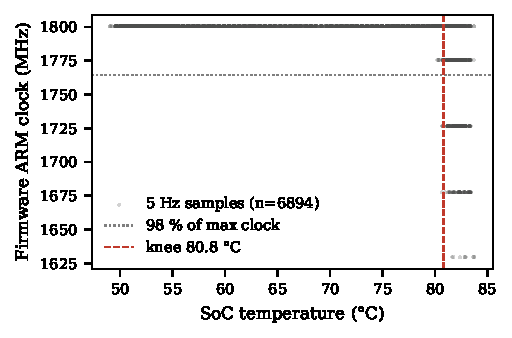
\includegraphics[width=\columnwidth]{figures/fig1_exp1_knee.pdf}
\caption{Experiment~1: firmware ARM clock against SoC temperature (6{,}894 samples at 5\,Hz, four-core load). The
knee (80.8\degC{}) is the lowest temperature at which the clock fell below 98\,\% of its maximum. Points are
jittered by $\pm0.15$\degC{} for visibility.}
\label{fig:knee}
\end{figure}

\subsection{G2: service time against temperature}\label{sec:g2}
In Experiment~2, run~3 (2 ramps, 3{,}027 HOT jobs, 36 kept bins), the OLS slope of bin-median latency on bin-median
temperature is \textbf{+0.208\,ms/\textdegree{}C} (95\,\% cluster-bootstrap CI [+0.070, +0.343]). G2 is
\textbf{PASS}.

The relationship is a step at the knee, not a line (Fig.~\ref{fig:sT}):
\begin{itemize}
\item \textbf{Below the knee:} bin medians stay within 196.23--196.55\,ms in all 30 bins, from 47.7 to 79.4\degC{}.
\item \textbf{Just above it:} 197.4--198.0\,ms at 81.3--81.8\degC{}.
\item \textbf{On the plateau:} 207.9--208.5\,ms at 83.3\degC{} and 211.0--212.1\,ms at 84.2\degC{}.
\end{itemize}

\begin{figure}[t]
\centering
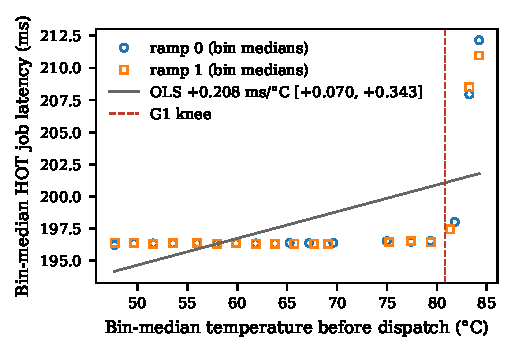
\includegraphics[width=\columnwidth]{figures/fig2_exp2_sT.pdf}
\caption{Experiment~2 (run~3): bin-median HOT job latency against bin-median temperature before dispatch (2\degC{}
bins, $\ge$20 jobs, two ramps). The preregistered OLS slope and its cluster-bootstrap CI summarise a step at the
80.8\degC{} knee.}
\label{fig:sT}
\end{figure}

\subsection{G3: cold-latency match}
In the accepted workload validation (40 pairs), median latency was 196.32\,ms for HOT and 196.22\,ms for COOL. The
gap is $-0.050$\,\% (95\,\% CI [$-0.080$, $-0.001$]\,\%), class TARGET MET. G3 is \textbf{PASS}.

\subsection{Session validity}
The Experiment~3 session ran 40 of 40 scheduled sequences in about 3\,h.
\begin{itemize}
\item All sequences were valid (10 per ordering), with no reruns.
\item No under-voltage was flagged, no watchdog signal was sent, and cleanup was verified.
\item Every sequence had exactly 300 HOT and 300 COOL jobs in its ordering's structure, and all 24{,}000 jobs
completed their planned units.
\end{itemize}
The A7 validity rule is met.

\subsection{G4: ordering and time above the knee}
Ordering changed the thermal trajectory (Fig.~\ref{fig:traj}, Fig.~\ref{fig:tak}, Table~\ref{tab:summary}):
\begin{itemize}
\item \code{hot\_first} ran up toward the knee during its HOT half.
\item \code{cool\_first} first cooled to about 61\degC{}, then climbed.
\item \code{alternating} and \code{random} settled near 71--72\degC{}.
\end{itemize}
Median time above the knee per sequence was 13.3\,s (\code{hot\_first}), 0.8\,s (\code{cool\_first}) and 0\,s
(\code{alternating}, \code{random}). The preregistered contrast between the largest and smallest median is
\textbf{+13.3\,s, 95\,\% CI [+6.0, +23.8]}. G4 is \textbf{PASS}.

\begin{figure}[t]
\centering
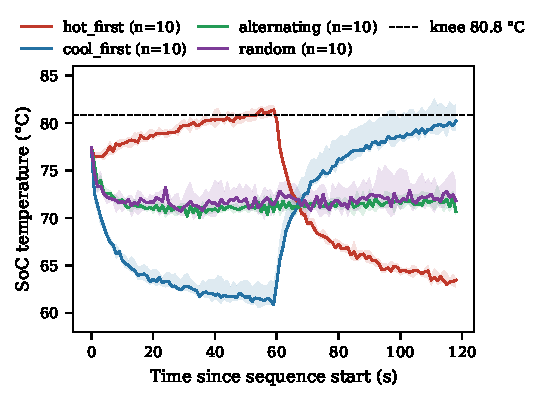
\includegraphics[width=\columnwidth]{figures/fig3_exp3_trajectories.pdf}
\caption{Experiment~3: SoC temperature during the 600-job sequences; median (line) and interquartile range (band)
across the 10 sequences of each ordering, aligned at sequence start.}
\label{fig:traj}
\end{figure}

\begin{figure}[t]
\centering
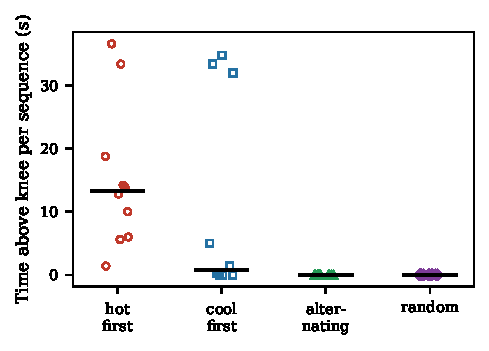
\includegraphics[width=\columnwidth]{figures/fig4_exp3_time_above_knee.pdf}
\caption{Experiment~3: time above the 80.8\degC{} knee per sequence (points) and per-ordering median (bar).}
\label{fig:tak}
\end{figure}

\begin{table*}[t]
\centering
\caption{Per-ordering summary, median [interquartile range] over 10 valid sequences each}
\label{tab:summary}
\footnotesize
\begin{tabular}{@{}lllll@{}}
\toprule
 & hot\_first & cool\_first & alternating & random\\
\midrule
Time above knee (s) & 13.3 [7.0, 17.7] & 0.8 [0.0, 25.3] & 0.0 [0.0, 0.0] & 0.0 [0.0, 0.0]\\
Peak temperature (\textdegree{}C) & 82.3 & 81.1 & 77.4 & 77.4\\
P99 latency (ms) & 201.26 [201.05, 201.61] & 201.35 [200.27, 207.60] & 202.14 [201.76, 202.42] & 201.51 [201.34, 201.83]\\
P95 latency (ms) & 199.39 & 199.44 & 199.40 & 199.34\\
Mean latency (ms) & 197.14 & 197.11 & 197.20 & 197.09\\
Throughput (jobs/s) & 5.014 & 5.015 & 5.013 & 5.015\\
\bottomrule
\end{tabular}
\end{table*}

\subsection{G5 and G5b: tail latency, mean latency, throughput}
Median per-sequence P99 differed by at most 0.88\,ms (0.44\,\%) between any two orderings (Fig.~\ref{fig:out},
Table~\ref{tab:pairs}).
\begin{itemize}
\item \textbf{Uncorrected:} one pair's CI excluded zero (\code{alternating} $-$ \code{random}, +0.62\,ms,
$p=0.046$).
\item \textbf{Holm:} with six pairs, Holm's first step needs $p\le0.0083$, so no pair survives. G5 is
\textbf{FAIL}.
\item \textbf{Secondary metrics:} for mean latency and throughput, the smallest $p$-values (0.037 and 0.045, the same
pair) also fail Holm's first step. G5b is \textbf{FAIL}.
\end{itemize}

\begin{figure*}[t]
\centering
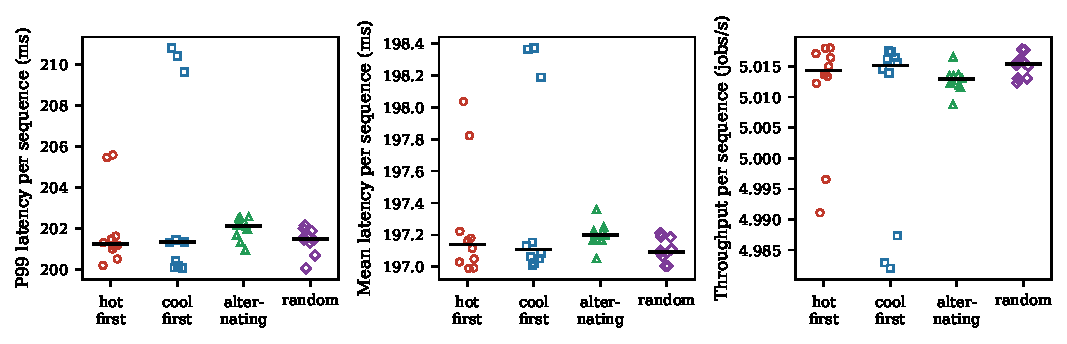
\includegraphics[width=\textwidth]{figures/fig5_exp3_outcomes.pdf}
\caption{Experiment~3: per-sequence P99 latency, mean latency and throughput by ordering (points; horizontal jitter
only), with medians (bars).}
\label{fig:out}
\end{figure*}

\begin{table}[t]
\centering
\caption{Pairwise differences in median per-sequence P99 (ms): bootstrap 95\,\% CI, two-sided bootstrap $p$, Holm
decision, Cliff's $\delta$}
\label{tab:pairs}
\footnotesize
\setlength{\tabcolsep}{3pt}
\begin{tabular}{@{}lrrrcr@{}}
\toprule
Pair & $\Delta$ & 95\,\% CI & $p$ & Holm & $\delta$\\
\midrule
alt $-$ cool & +0.79 & [$-7.66$, +1.97] & 0.306 & no & +0.30\\
alt $-$ hot & +0.88 & [$-1.29$, +1.36] & 0.068 & no & +0.44\\
alt $-$ rand & +0.62 & [+0.01, +1.08] & 0.046 & no & +0.56\\
cool $-$ hot & +0.09 & [$-1.97$, +8.45] & 0.979 & no & +0.00\\
cool $-$ rand & $-0.16$ & [$-1.39$, +8.18] & 0.389 & no & $-0.12$\\
hot $-$ rand & $-0.26$ & [$-0.75$, +1.90] & 0.340 & no & $-0.14$\\
\bottomrule
\end{tabular}
\end{table}

\subsection{G6 and verdict}
G6 is defined only if G4 and G5 both pass. Because G5 failed, G6 is \textbf{not testable}.

The committed analysis code, applied to the Experiment~1--3 records, returns G1--G4 PASS, G5 and G5b FAIL, and the
preregistered verdict \textbf{LIKELY KILL}: the thermal trajectory moves, but no performance metric responds.
Independently written code reproduces this verdict from the raw records.

\subsection{A thermal effect without a performance effect}\label{sec:discussion}
Ordering changed \emph{when} and \emph{for how long} the die was above its knee (G4). It did not move the latency
distribution enough to register in P99, mean latency or throughput (G5, G5b). The exploratory analyses below,
which cannot change the verdict, suggest why.

\textbf{At a two-minute horizon starting just below the knee, throttling is shallow.}
\begin{itemize}
\item Of 12{,}000 HOT jobs, 1{,}258 started at or above the knee. Their median latency was 198.29\,ms, against
196.87\,ms for HOT jobs below it (+0.7\,\%). Their 90th percentiles were 204.99 and 198.98\,ms.
\item The deeper clock reductions behind the 208--212\,ms plateau of Experiment~2 appear only after minutes of
continuous load. A \code{hot\_first} sequence runs at most 60\,s of HOT work.
\item In \code{hot\_first} sequences, a median 60 jobs per sequence (10\,\%) started at or above the knee, but most
of them were only slightly slower.
\end{itemize}

\subsection{What P99 measures for 600 jobs}\label{sec:p99}
Per sequence, P99 is in effect the 7th-largest of 600 latencies, and slow jobs are scarce:
\begin{itemize}
\item The median number of jobs slower than 205\,ms per sequence was 2.5, 2.5, 2.0 and 2.5 across orderings. The
number slower than 200\,ms was 14.5--18.
\item The 7th-largest latency is therefore usually an ordinary job of about 200--202\,ms, not a throttled one, in
every ordering.
\item The rare extreme outliers (11--15 jobs above 215\,ms per ordering, out of 6{,}000) mostly started below the
knee.
\item A job-level bootstrap within a sequence (assuming exchangeable jobs) gives a median 95\,\% interval width of
3.3\,ms for one sequence's P99.
\end{itemize}

\textbf{Sensitivity.} A rough normal approximation on the per-sequence P99 spread suggests that, with 10 sequences
per ordering and 80\,\% power at Holm's first step, detectable effects range from about 0.9\,ms
(\code{alternating} vs \code{random}) to 5.6\,ms (pairs involving \code{cool\_first}). The observed median
differences, $\le0.9$\,ms, are below most of these. A non-significant result is not equivalence. What the data
support is narrower: at this operating point, any ordering effect on the median per-sequence P99 is small relative
to a 196\,ms job, and the observed differences were under 0.5\,\%.

\subsection{Starting state and the session}
The preregistered design fixed a near-knee start (77\degC{}) and a two-minute horizon. Exploratory observations
show how much the outcome depends on thermal state (Fig.~\ref{fig:session}).

\textbf{Repetitions 0--2 (the first $\sim$70\,min):}
\begin{itemize}
\item Median cooldowns to 48.3\degC{} were 152, 217 and 262\,s, and median pre-heats 32--36\,s.
\item In 5 of the 6 \code{hot\_first} and \code{cool\_first} sequences, the die spent 32--37\,s above the knee, and
P99 was 205.5--210.8\,ms.
\item The \code{alternating} and \code{random} sequences of the same repetitions stayed at 200.1--202.6\,ms.
\end{itemize}

\textbf{Repetitions 3--9:} median cooldowns were 57--75\,s and median pre-heats 43--48\,s. P99 was
200.1--202.5\,ms in every ordering.

The cause is unknown; ambient temperature and airflow were not measured. Because every repetition contains all four
orderings, the shift adds variance rather than bias to the ordering comparison, and it produces the wide CIs for the
\code{cool\_first} pairs.

\textbf{A hypothesis, not a result.} When the device is loaded enough that blocked orderings spend more than about
30\,s above the knee within a sequence, ordering may move P99 by several milliseconds (2--5\,\%). That would need a
separately preregistered study with controlled ambient conditions.

\textbf{Pooling.} Pooling all 6{,}000 jobs of an ordering gives P99 values of 204.1, 207.9, 202.2 and 201.6\,ms
(Fig.~\ref{fig:ccdf}). These are dominated by the few hot early sequences. They are not the preregistered
statistic, but they show that the choice of summary changes the impression.

\begin{figure}[t]
\centering
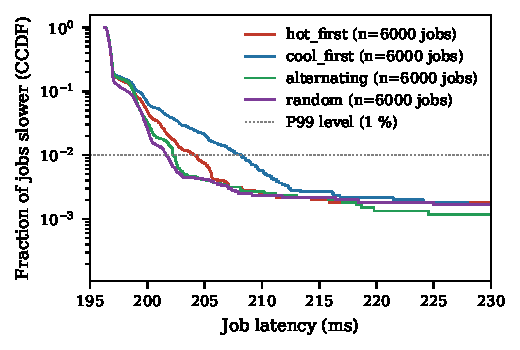
\includegraphics[width=\columnwidth]{figures/fig6_exp3_tail_ccdf_exploratory.pdf}
\caption{Exploratory: complementary CDF of job latency, all 6{,}000 jobs of each ordering (log scale). Not the
preregistered statistic; pooled tails are dominated by a few early-session sequences.}
\label{fig:ccdf}
\end{figure}

\begin{figure}[t]
\centering
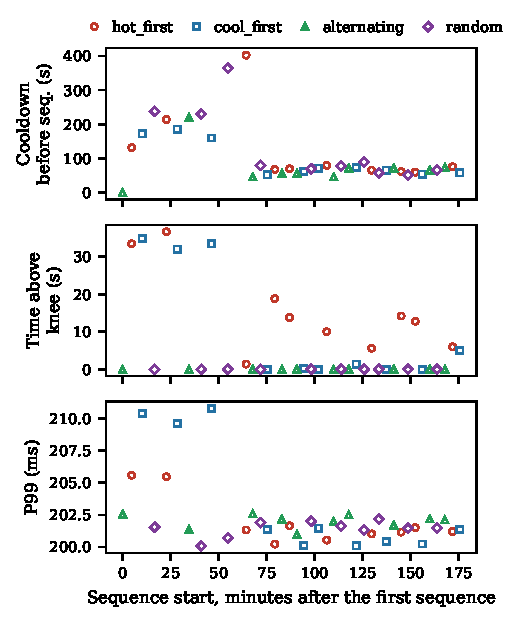
\includegraphics[width=\columnwidth]{figures/fig7_exp3_session_order_exploratory.pdf}
\caption{Exploratory: cooldown before each sequence, time above the knee, and P99 per sequence against session time.
The first $\sim$70\,min show long cooldowns and, for the blocked orderings, long times above the knee and higher
P99. (The first sequence needed no cooldown.)}
\label{fig:session}
\end{figure}

\subsection{Alternative explanations and supported claims}\label{sec:claims}
\textbf{Order effects.} Job-length differences are excluded within the validated tolerance (G3). Linear drift is
balanced by the schedule. Nonlinear drift is not excluded, but it is symmetric across orderings within each
repetition.

\textbf{Non-thermal outliers.} The extreme outliers above 215\,ms were spread evenly across orderings and mostly
started below the knee. This suggests operating-system or timing noise rather than throttling.

\textbf{Measurement perturbation.} The between-job flag reads and the 60\,s status observer were present in all
orderings alike.

\textbf{What we can and cannot conclude.}
\begin{itemize}
\item \textbf{Supported:} the causal claim that ordering changes time above the knee. The orderings were randomised
in order and the work was identical.
\item \textbf{Not supported:} the claim that ordering has \emph{no} effect on tail latency. The data allow small
effects, and larger ones in thermal states the session did not control.
\item \textbf{Physical versus practical:} the physical effect (G4) is real. A practically useful effect was not
observed.
\end{itemize}

\subsection{Limitations and threats to validity}\label{sec:limits}
\textbf{Generalisability.}
\begin{itemize}
\item One device and one environment; the bare-board configuration was confirmed afterwards, not logged on the day.
\item Ambient temperature was not measured.
\item One synthetic GEMM workload, without the memory, I/O or accelerator behaviour of real inference.
\item One sequence length (600 jobs) and one start band (77\degC{}); the protocol's sweep of three start
temperatures was not run.
\end{itemize}

\textbf{Power and percentile estimation.} Ten sequences per ordering cannot resolve sub-millisecond P99 effects.
P99 over 600 jobs rests on about 7 order statistics.

\textbf{Statistical assumptions.}
\begin{itemize}
\item The bootstrap assumes exchangeable sequences despite serial execution and a mid-session shift.
\item G4 compares a pair selected from the data, as preregistered.
\item Holm controls error within each metric only.
\end{itemize}

\textbf{Sensors.} The sensor is quantised at 0.487\degC{} and sampled at 5\,Hz. Time above the knee uses sysfs
temperature, not the firmware clock.

\textbf{Interference.} Between-job flag reads use a short-lived process, and a status observer polled every
60\,s. Both were present in all orderings.

\textbf{Process.} One amendment (A5) was approved under delegation before the experimenter reviewed it. Two Experiment~2
runs were inconclusive before G2 was decided. Both are disclosed.

\section{Conclusion and Future Scope}
On a passively cooled Raspberry Pi~4 running matched fixed-work four-core jobs, the order of an identical job
multiset changed how long the device spent above its throttling knee. At the preregistered operating point
(600-job sequences starting at 77\degC{}), that change did not produce a statistically supported difference in P99
latency, mean latency or throughput. The preregistered verdict is LIKELY KILL for the claim that ordering alone
improves tail latency on this device.

\textbf{Future scope.} The following are future experiments, not findings. Each needs its own preregistered
hypothesis, protocol and success criteria, and none can revise this verdict:
\begin{itemize}
\item longer hot blocks that reach the deep throttling plateau, within safety limits;
\item controlled initial thermal states and ambient conditions;
\item tail-sensitive designs sized by a power analysis from the variance reported here;
\item other devices, cooling configurations and real inference workloads.
\end{itemize}

\ifdefined\REVIEW\else
\section*{Author Contributions}
Srijan Srivastava carried out the research and prepared the paper. Padma Priya supervised the work and provided guidance.
\fi

\section*{Acknowledgment}
The authors used Claude (Anthropic), a generative AI assistant, throughout this work to help write and test the code, analyse the data, and draft the text and figures, and it approved amendment A5 under delegation; the authors reviewed the output and take full responsibility for the content.

\begin{thebibliography}{18}
\bibitem{brooks2001} D.~Brooks and M.~Martonosi, ``Dynamic thermal management for high-performance microprocessors,'' in \emph{Proc. 7th Int. Symp. High-Performance Computer Architecture (HPCA)}, 2001, pp. 171--182, doi: 10.1109/HPCA.2001.903261.
\bibitem{skadron2003} K.~Skadron, M.~R. Stan, W.~Huang, S.~Velusamy, K.~Sankaranarayanan, and D.~Tarjan, ``Temperature-aware microarchitecture,'' in \emph{Proc. 30th Annu. Int. Symp. Computer Architecture (ISCA)}, 2003, pp. 2--13, doi: 10.1145/859618.859620.
\bibitem{choi2007} J.~Choi, C.-Y. Cher, H.~Franke, H.~Hamann, A.~Weger, and P.~Bose, ``Thermal-aware task scheduling at the system software level,'' in \emph{Proc. Int. Symp. Low Power Electronics and Design (ISLPED)}, 2007, pp. 213--218, doi: 10.1145/1283780.1283826.
\bibitem{yang2008} J.~Yang, X.~Zhou, M.~Chrobak, Y.~Zhang, and L.~Jin, ``Dynamic thermal management through task scheduling,'' in \emph{Proc. IEEE Int. Symp. Performance Analysis of Systems and Software (ISPASS)}, 2008, pp. 191--201, doi: 10.1109/ISPASS.2008.4510751.
\bibitem{chrobak2008} M.~Chrobak, C.~D\"urr, M.~Hurand, and J.~Robert, ``Algorithms for temperature-aware task scheduling in microprocessor systems,'' in \emph{Algorithmic Aspects in Information and Management (AAIM)}, ser. Lecture Notes in Computer Science.\hskip 1em plus 0.5em minus 0.4em\relax Springer, 2008, pp. 120--130, doi: 10.1007/978-3-540-68880-8\_13.
\bibitem{coskun2008} A.~K. Coskun, T.~S. Rosing, K.~A. Whisnant, and K.~C. Gross, ``Static and dynamic temperature-aware scheduling for multiprocessor SoCs,'' \emph{IEEE Trans. Very Large Scale Integr. (VLSI) Syst.}, vol.~16, no.~9, pp. 1127--1140, 2008, doi: 10.1109/TVLSI.2008.2000726.
\bibitem{sahin2016} O.~Sahin and A.~K. Coskun, ``Providing sustainable performance in thermally constrained mobile devices,'' in \emph{Proc. 14th ACM/IEEE Symp. Embedded Systems for Real-Time Multimedia (ESTIMedia)}, 2016, pp. 72--77, doi: 10.1145/2993452.2994309.
\bibitem{rpi-thermal} Raspberry Pi Ltd, ``Raspberry Pi computer hardware: Frequency management and thermal control,'' Raspberry Pi Documentation. [Online]. Available: \url{https://www.raspberrypi.com/documentation/computers/raspberry-pi.html} (accessed Oct. 18, 2026).
\bibitem{rpi-throttled} Raspberry Pi Ltd, ``Raspberry Pi OS: vcgencmd get\_throttled,'' Raspberry Pi Documentation. [Online]. Available: \url{https://www.raspberrypi.com/documentation/computers/os.html} (accessed Oct. 18, 2026).
\bibitem{dean2013} J.~Dean and L.~A. Barroso, ``The tail at scale,'' \emph{Commun. ACM}, vol.~56, no.~2, pp. 74--80, 2013, doi: 10.1145/2408776.2408794.
\bibitem{zhang2016} Y.~Zhang, D.~Meisner, J.~Mars, and L.~Tang, ``Treadmill: Attributing the source of tail latency through precise load testing and statistical inference,'' in \emph{Proc. ACM/IEEE 43rd Annu. Int. Symp. Computer Architecture (ISCA)}, 2016, pp. 456--468, doi: 10.1109/ISCA.2016.47.
\bibitem{hyndman1996} R.~J. Hyndman and Y.~Fan, ``Sample quantiles in statistical packages,'' \emph{Amer. Statistician}, vol.~50, no.~4, pp. 361--365, 1996, doi: 10.1080/00031305.1996.10473566.
\bibitem{efron1979} B.~Efron, ``Bootstrap methods: Another look at the jackknife,'' \emph{Ann. Statist.}, vol.~7, no.~1, pp. 1--26, 1979, doi: 10.1214/aos/1176344552.
\bibitem{holm1979} S.~Holm, ``A simple sequentially rejective multiple test procedure,'' \emph{Scand. J. Statist.}, vol.~6, pp. 65--70, 1979. [Online]. Available: \url{https://www.jstor.org/stable/4615733}
\bibitem{cliff1993} N.~Cliff, ``Dominance statistics: Ordinal analyses to answer ordinal questions,'' \emph{Psychol. Bull.}, vol.~114, no.~3, pp. 494--509, 1993, doi: 10.1037/0033-2909.114.3.494.
\bibitem{hoefler2015} T.~Hoefler and R.~Belli, ``Scientific benchmarking of parallel computing systems: Twelve ways to tell the masses when reporting performance results,'' in \emph{Proc. Int. Conf. High Performance Computing, Networking, Storage and Analysis (SC)}, 2015, pp. 1--12, doi: 10.1145/2807591.2807644.
\bibitem{mytkowicz2009} T.~Mytkowicz, A.~Diwan, M.~Hauswirth, and P.~F. Sweeney, ``Producing wrong data without doing anything obviously wrong!'' in \emph{Proc. 14th Int. Conf. Architectural Support for Programming Languages and Operating Systems (ASPLOS)}, 2009, pp. 265--276, doi: 10.1145/1508244.1508275.
\bibitem{nosek2018} B.~A. Nosek, C.~R. Ebersole, A.~C. DeHaven, and D.~T. Mellor, ``The preregistration revolution,'' \emph{Proc. Natl. Acad. Sci. USA}, vol.~115, no.~11, pp. 2600--2606, 2018, doi: 10.1073/pnas.1708274114.
\end{thebibliography}

\end{document}
"
\ifdefined\REVIEW
\author{\IEEEauthorblockN{Anonymous Authors}
\IEEEauthorblockA{Names and affiliations withheld for double-blind review}}
\else
\author{\IEEEauthorblockN{Srijan Srivastava}
\IEEEauthorblockA{\textit{School of Computer Science and Engineering (SCOPE)}\\
\textit{Vellore Institute of Technology}\\
Vellore, India\\
\texttt{srijan.srivastava2023@vitstudent.ac.in}}
\and
\IEEEauthorblockN{Padma Priya}
\IEEEauthorblockA{\textit{School of Computer Science and Engineering (SCOPE)}\\
\textit{Vellore Institute of Technology}\\
Vellore, India\\
\texttt{padmapriya.r@vit.ac.in}}}
\fi

\maketitle

\begin{abstract}
On passively cooled edge devices, firmware throttles the CPU clock once the die is hot. One idea is to order
work so that heat-producing jobs are interleaved with lighter ones and fewer jobs run throttled. We tested whether
ordering alone changes tail latency. We used a Raspberry Pi~4 Model~B and a matched pair of fixed-work four-core
jobs, HOT (CPU duty 0.99) and COOL (0.38), whose cold latencies differ by $-0.05$\,\% (95\,\% CI
[$-0.08$, $-0.001$]\,\%). We compared four orderings of an identical 600-job multiset (hot-first, cool-first,
alternating, random), with 10 interleaved, counterbalanced repetitions each: 40 sequences and 24{,}000 jobs. Each
sequence started at 77.4--77.9\degC{} after a standardised cooldown and pre-heat. The hypotheses, gates and
analysis were preregistered. A throttle knee was found at 80.8\degC{} in the firmware ARM clock. Service time
rose with temperature (+0.208\,ms/\textdegree{}C, 95\,\% CI [+0.070, +0.343]): flat at about 196.4\,ms below the
knee and 208--212\,ms on the throttling plateau. Ordering changed the thermal trajectory: hot-first spent a median
13.3\,s above the knee per sequence, against 0\,s for alternating and random (difference 13.3\,s, CI [6.0, 23.8]).
It did not change tail latency: median per-sequence P99 ranged from 201.3 to 202.1\,ms across orderings, and no
pairwise difference survived Holm correction. Mean latency and throughput showed no supported difference either.
The preregistered verdict is LIKELY KILL. Exploratory analyses suggest why: throttling at this horizon is shallow,
and only about 2--3 of 600 jobs per sequence exceeded 205\,ms, so P99 is set by ordinary jobs. The device's
thermal state also shifted during the session. We report the negative result, its limits and the hypotheses it
leaves open.
\end{abstract}

\begin{IEEEkeywords}
thermal throttling, task ordering, tail latency, edge computing, Raspberry Pi, negative result, preregistration
\end{IEEEkeywords}

\section{Purpose and Objectives}
\subsection{Motivation}
Edge devices increasingly run sustained compute without active cooling. When their system-on-chip (SoC) heats up,
firmware lowers the CPU clock to stay within a thermal limit. On the Raspberry Pi~4, the vendor documents
progressive throttling of the Arm cores between 80 and 85\degC{}~\cite{rpi-thermal}. Thermal throttling has long
been studied as dynamic thermal management (DTM)~\cite{brooks2001,skadron2003}. Operating-system schedulers can
reduce thermal emergencies by choosing what runs when~\cite{choi2007,yang2008,coskun2008}. Order matters
physically: for a fixed set of tasks, the temperature reached depends on execution order~\cite{chrobak2008}.

Changing a device's thermal trajectory does not by itself change what an application observes. A throttled job is
slower only by the clock reduction it actually experiences, and a tail percentile moves only if enough jobs are
slowed by enough. A reordering that keeps the die below its knee for longer is therefore a \emph{candidate}
mechanism for lower tail latency, not evidence of it.

\subsection{Research question and objectives}
For an identical multiset of fixed-work jobs with matched cold latency, does the order
in which the jobs run change (a)~the time the device spends above its throttling knee, and (b)~the tail latency,
mean latency and throughput of the jobs?

We answer this with a preregistered, gate-based pilot on a Raspberry Pi~4, designed to falsify the idea cheaply.
Each gate's test and the verdict were fixed before the data that decided them. Every design change was recorded
as a dated amendment before the data it governed.

\textbf{Contributions} (limited to what the evidence shows):
\begin{enumerate}
\item A measured throttling knee (80.8\degC{}, firmware ARM clock) and service-time curve for this device and
workload. The Linux \code{scaling\_cur\_freq} interface did not show the throttling at all. Service time is flat
below the knee and steps up about 6--8\,\% on the throttling plateau (Sec.~\ref{sec:g1}, \ref{sec:g2}).
\item A preregistered ordering experiment with a negative primary outcome. Ordering changed the time above the
knee but produced no statistically supported change in P99, P95, mean latency or throughput at the tested
operating point. The verdict is LIKELY KILL (Sec.~\ref{sec:results}).
\item An exploratory analysis, kept separate from the confirmatory results, of why the thermal effect did not
reach the measured tail: shallow throttling at a two-minute horizon, the order statistic that a 600-job P99
measures, and a within-session shift of thermal state (Sec.~\ref{sec:discussion}--\ref{sec:claims}).
\item Disclosure of the measurement pitfalls met: an instrument blind spot, supervision that perturbed latency, and
a flawed early validity rule (Sec.~\ref{sec:integrity}).
\end{enumerate}
We propose no new scheduling algorithm and do not claim that ordering never matters. We tested one operating point
and found no supported performance effect there.

\subsection{Background and related work}
\textbf{Dynamic thermal management.} Brooks and Martonosi~\cite{brooks2001} studied DTM mechanisms that respond
when a processor nears its thermal limit. They argued that designing for typical rather than worst-case power is
possible with little performance loss. Skadron et al.~\cite{skadron2003} introduced the HotSpot model and runtime
techniques such as frequency scaling and migration. They noted that activity metrics are poor temperature proxies
and that sensor inaccuracy affects DTM. Our device uses firmware-controlled frequency reduction. The application
has no DVFS authority, which leaves ordering as one of the few levers available to software.

\textbf{Thermal-aware task scheduling.}
\begin{itemize}
\item Choi et al.~\cite{choi2007} exploited temporal and spatial ``heat slack'' through OS scheduling.
\item Yang et al.~\cite{yang2008} built a thermal-aware Linux job scheduler that exploits differences in thermal
behaviour among jobs. They reported 10.5--73.6\,\% fewer hardware DTM events and up to 7.6\,\% (average 4.1\,\%)
higher throughput.
\item Chrobak et al.~\cite{chrobak2008} formalised temperature-aware scheduling of unit jobs with heat
contributions.
\item Coskun et al.~\cite{coskun2008} reduced hot spots, gradients and thermal cycles on multiprocessor SoCs at
negligible performance cost.
\item On mobile devices, Sahin and Coskun~\cite{sahin2016} showed that throttling degrades QoS, and sustained
acceptable performance for up to $8\times$ longer.
\end{itemize}
These works establish that scheduling changes thermal behaviour, and on their platforms can change throughput or
QoS. Our study differs in four ways: it holds the \emph{work} fixed (matched jobs, differing only in order), it
uses \emph{tail latency} as the primary outcome, it runs on a low-cost single-board computer with firmware-only
DVFS, and it is preregistered with explicit kill criteria.

\textbf{Tail latency and its measurement.} Dean and Barroso~\cite{dean2013} explain why tail latency, not the mean,
governs the responsiveness of large services. Zhang et al.~\cite{zhang2016} show that tail measurements are
sensitive to load-testing methodology, and attribute tail sources by quantile regression. Sample percentiles have
several definitions~\cite{hyndman1996}; with 600 observations, a P99 rests on a handful of order statistics
(Sec.~\ref{sec:p99}). We use bootstrap intervals~\cite{efron1979}, Holm's correction~\cite{holm1979} and Cliff's
$\delta$~\cite{cliff1993}.

\textbf{Rigour and preregistration.} Hoefler and Belli~\cite{hoefler2015} give guidelines for reporting performance
results with appropriate statistics and confidence intervals. Mytkowicz et al.~\cite{mytkowicz2009} show how
innocuous setup changes bias measurements. Nosek et al.~\cite{nosek2018} argue for preregistration, which separates
confirmatory from exploratory analysis. We keep that separation throughout.

\textbf{Raspberry Pi thermal behaviour.} The official documentation describes the 80--85\degC{} throttling
range~\cite{rpi-thermal} and the \code{get\_throttled} status bits~\cite{rpi-throttled} that we use to detect
under-voltage and throttling. We found only informal vendor and hobbyist characterisations of Pi~4 cooling, not a
peer-reviewed study of job ordering against tail latency on this platform. Our search was limited, so this is not
a claim that none exists.

\section{Methodology and Approach}
\subsection{Hardware and software}
\begin{itemize}
\item \textbf{Device:} Raspberry Pi~4 Model~B Rev~1.4 (BCM2711, four Arm cores, \code{arm\_freq} 1800\,MHz,
1.8\,GiB usable memory).
\item \textbf{Software stack:} Debian~13; kernel 6.18.50+rpt-rpi-v8; firmware a8698392 (14 Sep 2026); governor
\code{performance} on all cores; no \code{temp\_limit} or \code{temp\_soft\_limit} override.
\item \textbf{Python:} 3.13.5 with NumPy 2.2.4 on the single-threaded Debian reference BLAS.
\item \textbf{Cooling:} a bare board with no heatsink or fan, in open air, as the protocol specifies. No
cooling device is registered with the kernel. The experimenter confirmed this configuration after the study; it
was not logged separately on the Experiment~3 day. Ambient temperature was not measured (Sec.~\ref{sec:limits}).
\end{itemize}

\subsection{Workload: matched fixed-work jobs}
A job uses all four cores at once: one worker per core (pinned) runs a fixed number of timed units. A unit is four
consecutive $128\times128$ single-precision matrix multiplications. Latency is measured from the dispatch of the
first shard to the reply of the last. The two job classes (frozen parameters \code{P4c-F1}) are:
\begin{itemize}
\item \textbf{HOT:} 13 units per core and no sleep (measured CPU duty 0.994).
\item \textbf{COOL:} 5 units per core with 119.55\,ms of sleep spread between them (duty 0.385).
\end{itemize}

A preregistered workload validation with 40 accepted HOT/COOL pairs accepted this pair:
\begin{itemize}
\item \textbf{Cold-latency match:} median HOT 196.32\,ms, COOL 196.22\,ms; relative gap $-0.050$\,\%, 95\,\% CI
[$-0.080$, $-0.001$]\,\%, within the preregistered $\pm2$\,\% target.
\item \textbf{Variability:} unit-time CV 0.83\,\%; HOT-latency CV 0.35\,\%.
\end{itemize}
The two classes therefore take the same time when cold but differ in heat produced. An identical multiset of them
can differ only in order. That is the manipulation: the same number of each class, the same planned units and the
same planned sleep. Energy was not measured.

\subsection{Orderings and sequences}
A sequence is 600 jobs, 300 HOT and 300 COOL, run back to back (119.6--120.4\,s). The four orderings use the
protocol's names:
\begin{itemize}
\item \code{hot\_first}: 300 HOT jobs, then 300 COOL jobs;
\item \code{cool\_first}: the reverse;
\item \code{alternating}: HOT and COOL in turn;
\item \code{random}: a new permutation for each sequence, from a seeded generator.
\end{itemize}

Each ordering was repeated 10 times. The 40 sequences were interleaved and counterbalanced: each repetition block
contains all four orderings, alternate blocks are reversed, then shuffled (seed~0).

Each sequence starts in three steps:
\begin{enumerate}
\item \textbf{Cooldown} with no load to idle\,+\,3\degC{} (48.3\degC{}), capped at 20\,min. The idle baseline,
45.28\degC{}, was measured at the start of the session.
\item \textbf{Pre-heat} with back-to-back HOT jobs, not recorded, until the temperature read before a job is at
least 77.0\degC{}. Capped at 5\,min.
\item \textbf{Sequence}, started immediately.
\end{enumerate}
Sequences started at 77.4--77.9\degC{}, just below the knee. The pre-heat took 31--53\,s.

\subsection{Measurement and supervision}
\textbf{Temperature.} SoC temperature was read from Linux sysfs (\code{thermal\_zone0}) by a 5\,Hz logger thread
during each sequence (23{,}843 samples), with readings quantised in steps of 0.487\degC{}.

\textbf{Per job.} We recorded the temperature just before dispatch, latency, CPU time and completed units. We also
recorded the firmware throttle flags (\code{vcgencmd get\_throttled}~\cite{rpi-throttled}), read between jobs and
outside the timed interval.

\textbf{What was not read live.} The firmware ARM clock was not read during Experiment~3. Live clock reads were
reserved for Experiment~2, because a stall control showed that they perturb a small fraction of jobs.

\textbf{Supervision.} An external watchdog whose loop starts no processes stops the run with a single SIGTERM at
85.0\degC{}, on under-voltage, or on failed readings. The experiment starts no load before it has verified the
watchdog. Workers are never killed with SIGKILL.

\subsection{Thermal knee}
The knee comes from a separate supervised Experiment~1 run: four HOT workers, 15\,min of continuous load, with the
cores 99.9--100\,\% busy. During it, the firmware ARM clock was read through \code{vcgencmd measure\_clock arm}. By
the preregistered definition, the knee is the lowest temperature at which the clock read below 98\,\% of the run's
maximum. Amendment A3 moved this measurement from \code{scaling\_cur\_freq} to the firmware clock before the run,
after an instrument check showed that \code{scaling\_cur\_freq} does not reflect firmware throttling on this device.

\subsection{Preregistered gates and verdict}
Table~\ref{tab:gates} lists the gates. Each was defined in the protocol or in Amendments A1--A7, before the data
it governs.

\textbf{Validity (A7).} G3--G6 are decided only by a completed, supervised session with P4c jobs, a G1 knee, and at
least 8 valid sequences per ordering. Otherwise they are INCONCLUSIVE.

\textbf{Verdict rule} (fixed before Experiment~3):
\begin{itemize}
\item a failure of a structural gate (G1, G2 or G4) is KILL;
\item G5 failing with a secondary metric responding is REFORMULATE;
\item G5 failing with no secondary response is \textbf{LIKELY KILL};
\item G1, G2, G4 and G5 all passing is PROCEED.
\end{itemize}

\begin{table*}[t]
\centering
\caption{Preregistered gates}
\label{tab:gates}
\footnotesize
\begin{tabular}{@{}l p{4.0cm} p{9.6cm} l@{}}
\toprule
Gate & Question & Test & Data\\
\midrule
G1 & Is there a throttle knee? & knee measured in a valid Exp.~1 run (A1, A3) & Exp.~1\\
G2 & Does service time depend on temperature? & OLS slope of bin-median latency on bin-median temperature; 2\degC{} bins per ramp with $\ge$20 jobs; cluster bootstrap over (ramp, bin), 2000 resamples; PASS if the 95\,\% CI $>0$ (A4) & Exp.~2\\
G3 & Are HOT and COOL indistinguishable when cold? & cold-latency gap within target in the accepted workload validation & validation\\
G4 & Does ordering change time above the knee? & largest minus smallest per-ordering median time above the knee; percentile bootstrap (10{,}000 resamples, seed 0); PASS if the 95\,\% CI excludes 0 & Exp.~3\\
G5 & Does ordering change tail latency? & 6 pairwise differences of median per-sequence P99; bootstrap $p$-values, Holm at $\alpha=0.05$ (A7); PASS if any pair survives & Exp.~3\\
G5b & Do secondary metrics respond? & the same for mean latency and throughput, Holm within each metric & Exp.~3\\
G6 & Is the effect mediated? & corr(time above knee, P99) $>0.3$, tested only if G4 and G5 pass & Exp.~3\\
\bottomrule
\end{tabular}
\end{table*}

\subsection{Statistics and unit of analysis}
\textbf{Unit of analysis.} The unit is the sequence: $n=10$ per ordering. Per-sequence P99 and P95 use NumPy's
default linear-interpolation percentile, Hyndman--Fan type~7~\cite{hyndman1996}. For 600 jobs, P99 is the
7th-largest latency, interpolated 1\,\% of the way toward the 6th largest.

\textbf{Differences.} Differences are differences of medians across sequences, with an unpaired percentile
bootstrap~\cite{efron1979}. The two-sided $p$-value is
$\min(1, 2\min(\Pr[\Delta^*\le 0], \Pr[\Delta^*\ge0]))$ over the 10{,}000 bootstrap differences~$\Delta^*$.
Effect sizes are the median difference in milliseconds and Cliff's $\delta$~\cite{cliff1993}.

\textbf{Independence.} The bootstrap treats an ordering's sequences as exchangeable. They were run serially on one
device. The interleaved, counterbalanced schedule protects the comparison from linear drift, but not from all time
dependence.

\textbf{Exploratory analyses.} Everything outside the gates is labelled exploratory and cannot change the verdict.

\subsection{Integrity checks and disclosed deviations}\label{sec:integrity}
\textbf{Integrity.} Every run archive is stored with its SHA-256 hash, which matches the copy on the device. Code on
the device was hash-pinned by the launcher. For this paper, independently written code recomputed every
per-sequence metric from the raw job and telemetry records; all matched the official record to within $10^{-6}$,
and the gate statistics and verdict reproduce exactly.

\textbf{Disclosed deviations and pitfalls:}
\begin{enumerate}
\item \textbf{Instrument blind spot.} \code{scaling\_cur\_freq} read 1800\,MHz in all 6{,}894 samples of the
Experiment~1 run, while the firmware clock fell to 1629\,MHz.
\item \textbf{Supervision perturbing the measurement.} An earlier four-core workload candidate was rejected on
latency variability. Diagnostics traced the variability to the external watchdog's process starts every 5\,s:
8~of~8 stalls fell on poll-overlapped jobs. The watchdog was rewritten to start no processes, and the accepted
configuration was validated under it.
\item \textbf{Validity-rule flaw.} The first Experiment~2 run was INCONCLUSIVE because a coverage rule could not be
met at four-core heating rates. The fix was a paced warm-up (A5), which was approved by the experimenter's
assistant under delegation and accepted by the experimenter afterwards.
\item \textbf{Safety stop.} The second Experiment~2 run was safety-stopped at 85.2\degC{}. A6 shortened each ramp.
\end{enumerate}
Both earlier Experiment~2 runs remain on record as INCONCLUSIVE, and G2 is decided by the third.

\section{Results and Findings}\label{sec:results}
\subsection{G1: throttle knee}\label{sec:g1}
In the Experiment~1 run (6{,}894 samples at 5\,Hz, no clock reading missing):
\begin{itemize}
\item The firmware ARM clock fell from 1800.5\,MHz to a minimum of 1629.4\,MHz, a depth of 9.5\,\%.
\item 477 samples were below 98\,\% of the maximum. The lowest temperature among them, the knee, was
\textbf{80.83\degC{}} (Fig.~\ref{fig:knee}), consistent with the vendor's 80--85\degC{} range~\cite{rpi-thermal}.
\item \code{scaling\_cur\_freq} never left 1800\,MHz.
\end{itemize}
G1 is \textbf{PASS}. The cooling time constant fitted in the run was 106.7\,s.

\begin{figure}[t]
\centering
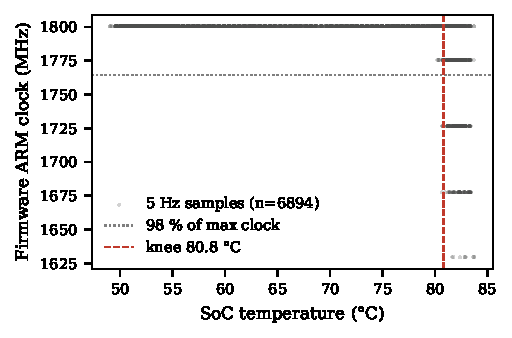
\includegraphics[width=\columnwidth]{figures/fig1_exp1_knee.pdf}
\caption{Experiment~1: firmware ARM clock against SoC temperature (6{,}894 samples at 5\,Hz, four-core load). The
knee (80.8\degC{}) is the lowest temperature at which the clock fell below 98\,\% of its maximum. Points are
jittered by $\pm0.15$\degC{} for visibility.}
\label{fig:knee}
\end{figure}

\subsection{G2: service time against temperature}\label{sec:g2}
In Experiment~2, run~3 (2 ramps, 3{,}027 HOT jobs, 36 kept bins), the OLS slope of bin-median latency on bin-median
temperature is \textbf{+0.208\,ms/\textdegree{}C} (95\,\% cluster-bootstrap CI [+0.070, +0.343]). G2 is
\textbf{PASS}.

The relationship is a step at the knee, not a line (Fig.~\ref{fig:sT}):
\begin{itemize}
\item \textbf{Below the knee:} bin medians stay within 196.23--196.55\,ms in all 30 bins, from 47.7 to 79.4\degC{}.
\item \textbf{Just above it:} 197.4--198.0\,ms at 81.3--81.8\degC{}.
\item \textbf{On the plateau:} 207.9--208.5\,ms at 83.3\degC{} and 211.0--212.1\,ms at 84.2\degC{}.
\end{itemize}

\begin{figure}[t]
\centering
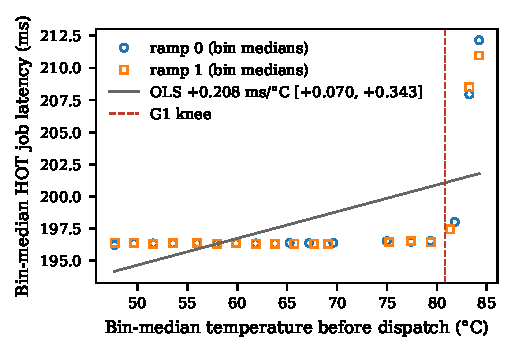
\includegraphics[width=\columnwidth]{figures/fig2_exp2_sT.pdf}
\caption{Experiment~2 (run~3): bin-median HOT job latency against bin-median temperature before dispatch (2\degC{}
bins, $\ge$20 jobs, two ramps). The preregistered OLS slope and its cluster-bootstrap CI summarise a step at the
80.8\degC{} knee.}
\label{fig:sT}
\end{figure}

\subsection{G3: cold-latency match}
In the accepted workload validation (40 pairs), median latency was 196.32\,ms for HOT and 196.22\,ms for COOL. The
gap is $-0.050$\,\% (95\,\% CI [$-0.080$, $-0.001$]\,\%), class TARGET MET. G3 is \textbf{PASS}.

\subsection{Session validity}
The Experiment~3 session ran 40 of 40 scheduled sequences in about 3\,h.
\begin{itemize}
\item All sequences were valid (10 per ordering), with no reruns.
\item No under-voltage was flagged, no watchdog signal was sent, and cleanup was verified.
\item Every sequence had exactly 300 HOT and 300 COOL jobs in its ordering's structure, and all 24{,}000 jobs
completed their planned units.
\end{itemize}
The A7 validity rule is met.

\subsection{G4: ordering and time above the knee}
Ordering changed the thermal trajectory (Fig.~\ref{fig:traj}, Fig.~\ref{fig:tak}, Table~\ref{tab:summary}):
\begin{itemize}
\item \code{hot\_first} ran up toward the knee during its HOT half.
\item \code{cool\_first} first cooled to about 61\degC{}, then climbed.
\item \code{alternating} and \code{random} settled near 71--72\degC{}.
\end{itemize}
Median time above the knee per sequence was 13.3\,s (\code{hot\_first}), 0.8\,s (\code{cool\_first}) and 0\,s
(\code{alternating}, \code{random}). The preregistered contrast between the largest and smallest median is
\textbf{+13.3\,s, 95\,\% CI [+6.0, +23.8]}. G4 is \textbf{PASS}.

\begin{figure}[t]
\centering
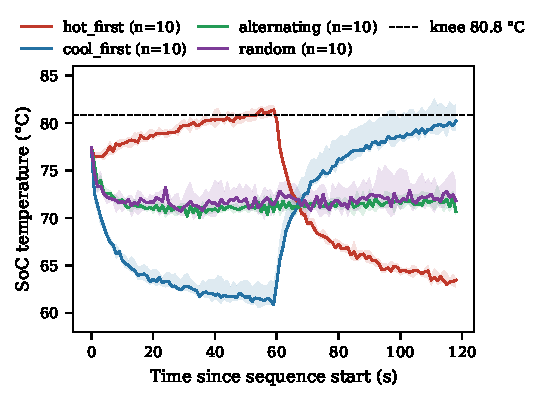
\includegraphics[width=\columnwidth]{figures/fig3_exp3_trajectories.pdf}
\caption{Experiment~3: SoC temperature during the 600-job sequences; median (line) and interquartile range (band)
across the 10 sequences of each ordering, aligned at sequence start.}
\label{fig:traj}
\end{figure}

\begin{figure}[t]
\centering
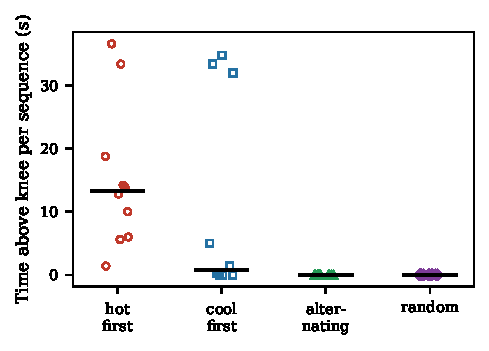
\includegraphics[width=\columnwidth]{figures/fig4_exp3_time_above_knee.pdf}
\caption{Experiment~3: time above the 80.8\degC{} knee per sequence (points) and per-ordering median (bar).}
\label{fig:tak}
\end{figure}

\begin{table*}[t]
\centering
\caption{Per-ordering summary, median [interquartile range] over 10 valid sequences each}
\label{tab:summary}
\footnotesize
\begin{tabular}{@{}lllll@{}}
\toprule
 & hot\_first & cool\_first & alternating & random\\
\midrule
Time above knee (s) & 13.3 [7.0, 17.7] & 0.8 [0.0, 25.3] & 0.0 [0.0, 0.0] & 0.0 [0.0, 0.0]\\
Peak temperature (\textdegree{}C) & 82.3 & 81.1 & 77.4 & 77.4\\
P99 latency (ms) & 201.26 [201.05, 201.61] & 201.35 [200.27, 207.60] & 202.14 [201.76, 202.42] & 201.51 [201.34, 201.83]\\
P95 latency (ms) & 199.39 & 199.44 & 199.40 & 199.34\\
Mean latency (ms) & 197.14 & 197.11 & 197.20 & 197.09\\
Throughput (jobs/s) & 5.014 & 5.015 & 5.013 & 5.015\\
\bottomrule
\end{tabular}
\end{table*}

\subsection{G5 and G5b: tail latency, mean latency, throughput}
Median per-sequence P99 differed by at most 0.88\,ms (0.44\,\%) between any two orderings (Fig.~\ref{fig:out},
Table~\ref{tab:pairs}).
\begin{itemize}
\item \textbf{Uncorrected:} one pair's CI excluded zero (\code{alternating} $-$ \code{random}, +0.62\,ms,
$p=0.046$).
\item \textbf{Holm:} with six pairs, Holm's first step needs $p\le0.0083$, so no pair survives. G5 is
\textbf{FAIL}.
\item \textbf{Secondary metrics:} for mean latency and throughput, the smallest $p$-values (0.037 and 0.045, the same
pair) also fail Holm's first step. G5b is \textbf{FAIL}.
\end{itemize}

\begin{figure*}[t]
\centering
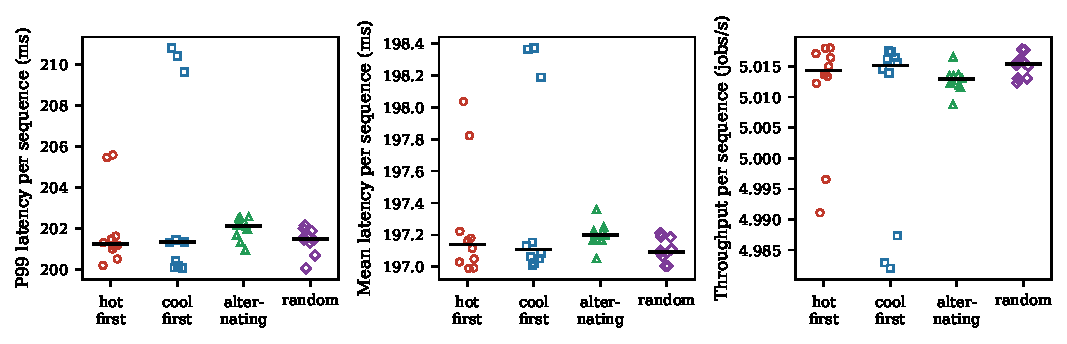
\includegraphics[width=\textwidth]{figures/fig5_exp3_outcomes.pdf}
\caption{Experiment~3: per-sequence P99 latency, mean latency and throughput by ordering (points; horizontal jitter
only), with medians (bars).}
\label{fig:out}
\end{figure*}

\begin{table}[t]
\centering
\caption{Pairwise differences in median per-sequence P99 (ms): bootstrap 95\,\% CI, two-sided bootstrap $p$, Holm
decision, Cliff's $\delta$}
\label{tab:pairs}
\footnotesize
\setlength{\tabcolsep}{3pt}
\begin{tabular}{@{}lrrrcr@{}}
\toprule
Pair & $\Delta$ & 95\,\% CI & $p$ & Holm & $\delta$\\
\midrule
alt $-$ cool & +0.79 & [$-7.66$, +1.97] & 0.306 & no & +0.30\\
alt $-$ hot & +0.88 & [$-1.29$, +1.36] & 0.068 & no & +0.44\\
alt $-$ rand & +0.62 & [+0.01, +1.08] & 0.046 & no & +0.56\\
cool $-$ hot & +0.09 & [$-1.97$, +8.45] & 0.979 & no & +0.00\\
cool $-$ rand & $-0.16$ & [$-1.39$, +8.18] & 0.389 & no & $-0.12$\\
hot $-$ rand & $-0.26$ & [$-0.75$, +1.90] & 0.340 & no & $-0.14$\\
\bottomrule
\end{tabular}
\end{table}

\subsection{G6 and verdict}
G6 is defined only if G4 and G5 both pass. Because G5 failed, G6 is \textbf{not testable}.

The committed analysis code, applied to the Experiment~1--3 records, returns G1--G4 PASS, G5 and G5b FAIL, and the
preregistered verdict \textbf{LIKELY KILL}: the thermal trajectory moves, but no performance metric responds.
Independently written code reproduces this verdict from the raw records.

\subsection{A thermal effect without a performance effect}\label{sec:discussion}
Ordering changed \emph{when} and \emph{for how long} the die was above its knee (G4). It did not move the latency
distribution enough to register in P99, mean latency or throughput (G5, G5b). The exploratory analyses below,
which cannot change the verdict, suggest why.

\textbf{At a two-minute horizon starting just below the knee, throttling is shallow.}
\begin{itemize}
\item Of 12{,}000 HOT jobs, 1{,}258 started at or above the knee. Their median latency was 198.29\,ms, against
196.87\,ms for HOT jobs below it (+0.7\,\%). Their 90th percentiles were 204.99 and 198.98\,ms.
\item The deeper clock reductions behind the 208--212\,ms plateau of Experiment~2 appear only after minutes of
continuous load. A \code{hot\_first} sequence runs at most 60\,s of HOT work.
\item In \code{hot\_first} sequences, a median 60 jobs per sequence (10\,\%) started at or above the knee, but most
of them were only slightly slower.
\end{itemize}

\subsection{What P99 measures for 600 jobs}\label{sec:p99}
Per sequence, P99 is in effect the 7th-largest of 600 latencies, and slow jobs are scarce:
\begin{itemize}
\item The median number of jobs slower than 205\,ms per sequence was 2.5, 2.5, 2.0 and 2.5 across orderings. The
number slower than 200\,ms was 14.5--18.
\item The 7th-largest latency is therefore usually an ordinary job of about 200--202\,ms, not a throttled one, in
every ordering.
\item The rare extreme outliers (11--15 jobs above 215\,ms per ordering, out of 6{,}000) mostly started below the
knee.
\item A job-level bootstrap within a sequence (assuming exchangeable jobs) gives a median 95\,\% interval width of
3.3\,ms for one sequence's P99.
\end{itemize}

\textbf{Sensitivity.} A rough normal approximation on the per-sequence P99 spread suggests that, with 10 sequences
per ordering and 80\,\% power at Holm's first step, detectable effects range from about 0.9\,ms
(\code{alternating} vs \code{random}) to 5.6\,ms (pairs involving \code{cool\_first}). The observed median
differences, $\le0.9$\,ms, are below most of these. A non-significant result is not equivalence. What the data
support is narrower: at this operating point, any ordering effect on the median per-sequence P99 is small relative
to a 196\,ms job, and the observed differences were under 0.5\,\%.

\subsection{Starting state and the session}
The preregistered design fixed a near-knee start (77\degC{}) and a two-minute horizon. Exploratory observations
show how much the outcome depends on thermal state (Fig.~\ref{fig:session}).

\textbf{Repetitions 0--2 (the first $\sim$70\,min):}
\begin{itemize}
\item Median cooldowns to 48.3\degC{} were 152, 217 and 262\,s, and median pre-heats 32--36\,s.
\item In 5 of the 6 \code{hot\_first} and \code{cool\_first} sequences, the die spent 32--37\,s above the knee, and
P99 was 205.5--210.8\,ms.
\item The \code{alternating} and \code{random} sequences of the same repetitions stayed at 200.1--202.6\,ms.
\end{itemize}

\textbf{Repetitions 3--9:} median cooldowns were 57--75\,s and median pre-heats 43--48\,s. P99 was
200.1--202.5\,ms in every ordering.

The cause is unknown; ambient temperature and airflow were not measured. Because every repetition contains all four
orderings, the shift adds variance rather than bias to the ordering comparison, and it produces the wide CIs for the
\code{cool\_first} pairs.

\textbf{A hypothesis, not a result.} When the device is loaded enough that blocked orderings spend more than about
30\,s above the knee within a sequence, ordering may move P99 by several milliseconds (2--5\,\%). That would need a
separately preregistered study with controlled ambient conditions.

\textbf{Pooling.} Pooling all 6{,}000 jobs of an ordering gives P99 values of 204.1, 207.9, 202.2 and 201.6\,ms
(Fig.~\ref{fig:ccdf}). These are dominated by the few hot early sequences. They are not the preregistered
statistic, but they show that the choice of summary changes the impression.

\begin{figure}[t]
\centering
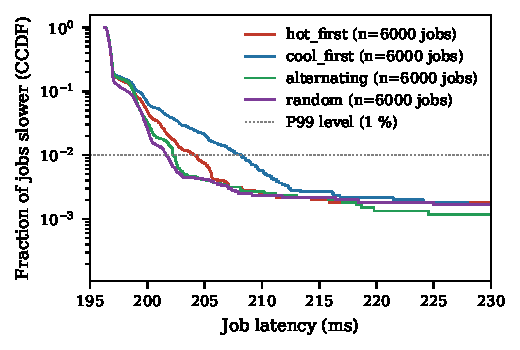
\includegraphics[width=\columnwidth]{figures/fig6_exp3_tail_ccdf_exploratory.pdf}
\caption{Exploratory: complementary CDF of job latency, all 6{,}000 jobs of each ordering (log scale). Not the
preregistered statistic; pooled tails are dominated by a few early-session sequences.}
\label{fig:ccdf}
\end{figure}

\begin{figure}[t]
\centering
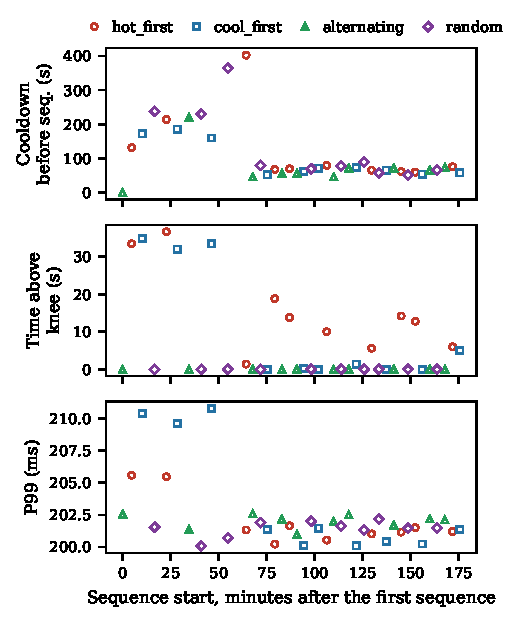
\includegraphics[width=\columnwidth]{figures/fig7_exp3_session_order_exploratory.pdf}
\caption{Exploratory: cooldown before each sequence, time above the knee, and P99 per sequence against session time.
The first $\sim$70\,min show long cooldowns and, for the blocked orderings, long times above the knee and higher
P99. (The first sequence needed no cooldown.)}
\label{fig:session}
\end{figure}

\subsection{Alternative explanations and supported claims}\label{sec:claims}
\textbf{Order effects.} Job-length differences are excluded within the validated tolerance (G3). Linear drift is
balanced by the schedule. Nonlinear drift is not excluded, but it is symmetric across orderings within each
repetition.

\textbf{Non-thermal outliers.} The extreme outliers above 215\,ms were spread evenly across orderings and mostly
started below the knee. This suggests operating-system or timing noise rather than throttling.

\textbf{Measurement perturbation.} The between-job flag reads and the 60\,s status observer were present in all
orderings alike.

\textbf{What we can and cannot conclude.}
\begin{itemize}
\item \textbf{Supported:} the causal claim that ordering changes time above the knee. The orderings were randomised
in order and the work was identical.
\item \textbf{Not supported:} the claim that ordering has \emph{no} effect on tail latency. The data allow small
effects, and larger ones in thermal states the session did not control.
\item \textbf{Physical versus practical:} the physical effect (G4) is real. A practically useful effect was not
observed.
\end{itemize}

\subsection{Limitations and threats to validity}\label{sec:limits}
\textbf{Generalisability.}
\begin{itemize}
\item One device and one environment; the bare-board configuration was confirmed afterwards, not logged on the day.
\item Ambient temperature was not measured.
\item One synthetic GEMM workload, without the memory, I/O or accelerator behaviour of real inference.
\item One sequence length (600 jobs) and one start band (77\degC{}); the protocol's sweep of three start
temperatures was not run.
\end{itemize}

\textbf{Power and percentile estimation.} Ten sequences per ordering cannot resolve sub-millisecond P99 effects.
P99 over 600 jobs rests on about 7 order statistics.

\textbf{Statistical assumptions.}
\begin{itemize}
\item The bootstrap assumes exchangeable sequences despite serial execution and a mid-session shift.
\item G4 compares a pair selected from the data, as preregistered.
\item Holm controls error within each metric only.
\end{itemize}

\textbf{Sensors.} The sensor is quantised at 0.487\degC{} and sampled at 5\,Hz. Time above the knee uses sysfs
temperature, not the firmware clock.

\textbf{Interference.} Between-job flag reads use a short-lived process, and a status observer polled every
60\,s. Both were present in all orderings.

\textbf{Process.} One amendment (A5) was approved under delegation before the experimenter reviewed it. Two Experiment~2
runs were inconclusive before G2 was decided. Both are disclosed.

\section{Conclusion and Future Scope}
On a passively cooled Raspberry Pi~4 running matched fixed-work four-core jobs, the order of an identical job
multiset changed how long the device spent above its throttling knee. At the preregistered operating point
(600-job sequences starting at 77\degC{}), that change did not produce a statistically supported difference in P99
latency, mean latency or throughput. The preregistered verdict is LIKELY KILL for the claim that ordering alone
improves tail latency on this device.

\textbf{Future scope.} The following are future experiments, not findings. Each needs its own preregistered
hypothesis, protocol and success criteria, and none can revise this verdict:
\begin{itemize}
\item longer hot blocks that reach the deep throttling plateau, within safety limits;
\item controlled initial thermal states and ambient conditions;
\item tail-sensitive designs sized by a power analysis from the variance reported here;
\item other devices, cooling configurations and real inference workloads.
\end{itemize}

\ifdefined\REVIEW\else
\section*{Author Contributions}
Srijan Srivastava carried out the research and prepared the paper. Padma Priya supervised the work and provided guidance.
\fi

\section*{Acknowledgment}
The authors used Claude (Anthropic), a generative AI assistant, throughout this work to help write and test the code, analyse the data, and draft the text and figures, and it approved amendment A5 under delegation; the authors reviewed the output and take full responsibility for the content.

\begin{thebibliography}{18}
\bibitem{brooks2001} D.~Brooks and M.~Martonosi, ``Dynamic thermal management for high-performance microprocessors,'' in \emph{Proc. 7th Int. Symp. High-Performance Computer Architecture (HPCA)}, 2001, pp. 171--182, doi: 10.1109/HPCA.2001.903261.
\bibitem{skadron2003} K.~Skadron, M.~R. Stan, W.~Huang, S.~Velusamy, K.~Sankaranarayanan, and D.~Tarjan, ``Temperature-aware microarchitecture,'' in \emph{Proc. 30th Annu. Int. Symp. Computer Architecture (ISCA)}, 2003, pp. 2--13, doi: 10.1145/859618.859620.
\bibitem{choi2007} J.~Choi, C.-Y. Cher, H.~Franke, H.~Hamann, A.~Weger, and P.~Bose, ``Thermal-aware task scheduling at the system software level,'' in \emph{Proc. Int. Symp. Low Power Electronics and Design (ISLPED)}, 2007, pp. 213--218, doi: 10.1145/1283780.1283826.
\bibitem{yang2008} J.~Yang, X.~Zhou, M.~Chrobak, Y.~Zhang, and L.~Jin, ``Dynamic thermal management through task scheduling,'' in \emph{Proc. IEEE Int. Symp. Performance Analysis of Systems and Software (ISPASS)}, 2008, pp. 191--201, doi: 10.1109/ISPASS.2008.4510751.
\bibitem{chrobak2008} M.~Chrobak, C.~D\"urr, M.~Hurand, and J.~Robert, ``Algorithms for temperature-aware task scheduling in microprocessor systems,'' in \emph{Algorithmic Aspects in Information and Management (AAIM)}, ser. Lecture Notes in Computer Science.\hskip 1em plus 0.5em minus 0.4em\relax Springer, 2008, pp. 120--130, doi: 10.1007/978-3-540-68880-8\_13.
\bibitem{coskun2008} A.~K. Coskun, T.~S. Rosing, K.~A. Whisnant, and K.~C. Gross, ``Static and dynamic temperature-aware scheduling for multiprocessor SoCs,'' \emph{IEEE Trans. Very Large Scale Integr. (VLSI) Syst.}, vol.~16, no.~9, pp. 1127--1140, 2008, doi: 10.1109/TVLSI.2008.2000726.
\bibitem{sahin2016} O.~Sahin and A.~K. Coskun, ``Providing sustainable performance in thermally constrained mobile devices,'' in \emph{Proc. 14th ACM/IEEE Symp. Embedded Systems for Real-Time Multimedia (ESTIMedia)}, 2016, pp. 72--77, doi: 10.1145/2993452.2994309.
\bibitem{rpi-thermal} Raspberry Pi Ltd, ``Raspberry Pi computer hardware: Frequency management and thermal control,'' Raspberry Pi Documentation. [Online]. Available: \url{https://www.raspberrypi.com/documentation/computers/raspberry-pi.html} (accessed Oct. 18, 2026).
\bibitem{rpi-throttled} Raspberry Pi Ltd, ``Raspberry Pi OS: vcgencmd get\_throttled,'' Raspberry Pi Documentation. [Online]. Available: \url{https://www.raspberrypi.com/documentation/computers/os.html} (accessed Oct. 18, 2026).
\bibitem{dean2013} J.~Dean and L.~A. Barroso, ``The tail at scale,'' \emph{Commun. ACM}, vol.~56, no.~2, pp. 74--80, 2013, doi: 10.1145/2408776.2408794.
\bibitem{zhang2016} Y.~Zhang, D.~Meisner, J.~Mars, and L.~Tang, ``Treadmill: Attributing the source of tail latency through precise load testing and statistical inference,'' in \emph{Proc. ACM/IEEE 43rd Annu. Int. Symp. Computer Architecture (ISCA)}, 2016, pp. 456--468, doi: 10.1109/ISCA.2016.47.
\bibitem{hyndman1996} R.~J. Hyndman and Y.~Fan, ``Sample quantiles in statistical packages,'' \emph{Amer. Statistician}, vol.~50, no.~4, pp. 361--365, 1996, doi: 10.1080/00031305.1996.10473566.
\bibitem{efron1979} B.~Efron, ``Bootstrap methods: Another look at the jackknife,'' \emph{Ann. Statist.}, vol.~7, no.~1, pp. 1--26, 1979, doi: 10.1214/aos/1176344552.
\bibitem{holm1979} S.~Holm, ``A simple sequentially rejective multiple test procedure,'' \emph{Scand. J. Statist.}, vol.~6, pp. 65--70, 1979. [Online]. Available: \url{https://www.jstor.org/stable/4615733}
\bibitem{cliff1993} N.~Cliff, ``Dominance statistics: Ordinal analyses to answer ordinal questions,'' \emph{Psychol. Bull.}, vol.~114, no.~3, pp. 494--509, 1993, doi: 10.1037/0033-2909.114.3.494.
\bibitem{hoefler2015} T.~Hoefler and R.~Belli, ``Scientific benchmarking of parallel computing systems: Twelve ways to tell the masses when reporting performance results,'' in \emph{Proc. Int. Conf. High Performance Computing, Networking, Storage and Analysis (SC)}, 2015, pp. 1--12, doi: 10.1145/2807591.2807644.
\bibitem{mytkowicz2009} T.~Mytkowicz, A.~Diwan, M.~Hauswirth, and P.~F. Sweeney, ``Producing wrong data without doing anything obviously wrong!'' in \emph{Proc. 14th Int. Conf. Architectural Support for Programming Languages and Operating Systems (ASPLOS)}, 2009, pp. 265--276, doi: 10.1145/1508244.1508275.
\bibitem{nosek2018} B.~A. Nosek, C.~R. Ebersole, A.~C. DeHaven, and D.~T. Mellor, ``The preregistration revolution,'' \emph{Proc. Natl. Acad. Sci. USA}, vol.~115, no.~11, pp. 2600--2606, 2018, doi: 10.1073/pnas.1708274114.
\end{thebibliography}

\end{document}
"
\ifdefined\REVIEW
\author{\IEEEauthorblockN{Anonymous Authors}
\IEEEauthorblockA{Names and affiliations withheld for double-blind review}}
\else
\author{\IEEEauthorblockN{Srijan Srivastava}
\IEEEauthorblockA{\textit{School of Computer Science and Engineering (SCOPE)}\\
\textit{Vellore Institute of Technology}\\
Vellore, India\\
\texttt{srijan.srivastava2023@vitstudent.ac.in}}
\and
\IEEEauthorblockN{Padma Priya}
\IEEEauthorblockA{\textit{School of Computer Science and Engineering (SCOPE)}\\
\textit{Vellore Institute of Technology}\\
Vellore, India\\
\texttt{padmapriya.r@vit.ac.in}}}
\fi

\maketitle

\begin{abstract}
On passively cooled edge devices, firmware throttles the CPU clock once the die is hot. One idea is to order
work so that heat-producing jobs are interleaved with lighter ones and fewer jobs run throttled. We tested whether
ordering alone changes tail latency. We used a Raspberry Pi~4 Model~B and a matched pair of fixed-work four-core
jobs, HOT (CPU duty 0.99) and COOL (0.38), whose cold latencies differ by $-0.05$\,\% (95\,\% CI
[$-0.08$, $-0.001$]\,\%). We compared four orderings of an identical 600-job multiset (hot-first, cool-first,
alternating, random), with 10 interleaved, counterbalanced repetitions each: 40 sequences and 24{,}000 jobs. Each
sequence started at 77.4--77.9\degC{} after a standardised cooldown and pre-heat. The hypotheses, gates and
analysis were preregistered. A throttle knee was found at 80.8\degC{} in the firmware ARM clock. Service time
rose with temperature (+0.208\,ms/\textdegree{}C, 95\,\% CI [+0.070, +0.343]): flat at about 196.4\,ms below the
knee and 208--212\,ms on the throttling plateau. Ordering changed the thermal trajectory: hot-first spent a median
13.3\,s above the knee per sequence, against 0\,s for alternating and random (difference 13.3\,s, CI [6.0, 23.8]).
It did not change tail latency: median per-sequence P99 ranged from 201.3 to 202.1\,ms across orderings, and no
pairwise difference survived Holm correction. Mean latency and throughput showed no supported difference either.
The preregistered verdict is LIKELY KILL. Exploratory analyses suggest why: throttling at this horizon is shallow,
and only about 2--3 of 600 jobs per sequence exceeded 205\,ms, so P99 is set by ordinary jobs. The device's
thermal state also shifted during the session. We report the negative result, its limits and the hypotheses it
leaves open.
\end{abstract}

\begin{IEEEkeywords}
thermal throttling, task ordering, tail latency, edge computing, Raspberry Pi, negative result, preregistration
\end{IEEEkeywords}

\section{Purpose and Objectives}
\subsection{Motivation}
Edge devices increasingly run sustained compute without active cooling. When their system-on-chip (SoC) heats up,
firmware lowers the CPU clock to stay within a thermal limit. On the Raspberry Pi~4, the vendor documents
progressive throttling of the Arm cores between 80 and 85\degC{}~\cite{rpi-thermal}. Thermal throttling has long
been studied as dynamic thermal management (DTM)~\cite{brooks2001,skadron2003}. Operating-system schedulers can
reduce thermal emergencies by choosing what runs when~\cite{choi2007,yang2008,coskun2008}. Order matters
physically: for a fixed set of tasks, the temperature reached depends on execution order~\cite{chrobak2008}.

Changing a device's thermal trajectory does not by itself change what an application observes. A throttled job is
slower only by the clock reduction it actually experiences, and a tail percentile moves only if enough jobs are
slowed by enough. A reordering that keeps the die below its knee for longer is therefore a \emph{candidate}
mechanism for lower tail latency, not evidence of it.

\subsection{Research question and objectives}
For an identical multiset of fixed-work jobs with matched cold latency, does the order
in which the jobs run change (a)~the time the device spends above its throttling knee, and (b)~the tail latency,
mean latency and throughput of the jobs?

We answer this with a preregistered, gate-based pilot on a Raspberry Pi~4, designed to falsify the idea cheaply.
Each gate's test and the verdict were fixed before the data that decided them. Every design change was recorded
as a dated amendment before the data it governed.

\textbf{Contributions} (limited to what the evidence shows):
\begin{enumerate}
\item A measured throttling knee (80.8\degC{}, firmware ARM clock) and service-time curve for this device and
workload. The Linux \code{scaling\_cur\_freq} interface did not show the throttling at all. Service time is flat
below the knee and steps up about 6--8\,\% on the throttling plateau (Sec.~\ref{sec:g1}, \ref{sec:g2}).
\item A preregistered ordering experiment with a negative primary outcome. Ordering changed the time above the
knee but produced no statistically supported change in P99, P95, mean latency or throughput at the tested
operating point. The verdict is LIKELY KILL (Sec.~\ref{sec:results}).
\item An exploratory analysis, kept separate from the confirmatory results, of why the thermal effect did not
reach the measured tail: shallow throttling at a two-minute horizon, the order statistic that a 600-job P99
measures, and a within-session shift of thermal state (Sec.~\ref{sec:discussion}--\ref{sec:claims}).
\item Disclosure of the measurement pitfalls met: an instrument blind spot, supervision that perturbed latency, and
a flawed early validity rule (Sec.~\ref{sec:integrity}).
\end{enumerate}
We propose no new scheduling algorithm and do not claim that ordering never matters. We tested one operating point
and found no supported performance effect there.

\subsection{Background and related work}
\textbf{Dynamic thermal management.} Brooks and Martonosi~\cite{brooks2001} studied DTM mechanisms that respond
when a processor nears its thermal limit. They argued that designing for typical rather than worst-case power is
possible with little performance loss. Skadron et al.~\cite{skadron2003} introduced the HotSpot model and runtime
techniques such as frequency scaling and migration. They noted that activity metrics are poor temperature proxies
and that sensor inaccuracy affects DTM. Our device uses firmware-controlled frequency reduction. The application
has no DVFS authority, which leaves ordering as one of the few levers available to software.

\textbf{Thermal-aware task scheduling.}
\begin{itemize}
\item Choi et al.~\cite{choi2007} exploited temporal and spatial ``heat slack'' through OS scheduling.
\item Yang et al.~\cite{yang2008} built a thermal-aware Linux job scheduler that exploits differences in thermal
behaviour among jobs. They reported 10.5--73.6\,\% fewer hardware DTM events and up to 7.6\,\% (average 4.1\,\%)
higher throughput.
\item Chrobak et al.~\cite{chrobak2008} formalised temperature-aware scheduling of unit jobs with heat
contributions.
\item Coskun et al.~\cite{coskun2008} reduced hot spots, gradients and thermal cycles on multiprocessor SoCs at
negligible performance cost.
\item On mobile devices, Sahin and Coskun~\cite{sahin2016} showed that throttling degrades QoS, and sustained
acceptable performance for up to $8\times$ longer.
\end{itemize}
These works establish that scheduling changes thermal behaviour, and on their platforms can change throughput or
QoS. Our study differs in four ways: it holds the \emph{work} fixed (matched jobs, differing only in order), it
uses \emph{tail latency} as the primary outcome, it runs on a low-cost single-board computer with firmware-only
DVFS, and it is preregistered with explicit kill criteria.

\textbf{Tail latency and its measurement.} Dean and Barroso~\cite{dean2013} explain why tail latency, not the mean,
governs the responsiveness of large services. Zhang et al.~\cite{zhang2016} show that tail measurements are
sensitive to load-testing methodology, and attribute tail sources by quantile regression. Sample percentiles have
several definitions~\cite{hyndman1996}; with 600 observations, a P99 rests on a handful of order statistics
(Sec.~\ref{sec:p99}). We use bootstrap intervals~\cite{efron1979}, Holm's correction~\cite{holm1979} and Cliff's
$\delta$~\cite{cliff1993}.

\textbf{Rigour and preregistration.} Hoefler and Belli~\cite{hoefler2015} give guidelines for reporting performance
results with appropriate statistics and confidence intervals. Mytkowicz et al.~\cite{mytkowicz2009} show how
innocuous setup changes bias measurements. Nosek et al.~\cite{nosek2018} argue for preregistration, which separates
confirmatory from exploratory analysis. We keep that separation throughout.

\textbf{Raspberry Pi thermal behaviour.} The official documentation describes the 80--85\degC{} throttling
range~\cite{rpi-thermal} and the \code{get\_throttled} status bits~\cite{rpi-throttled} that we use to detect
under-voltage and throttling. We found only informal vendor and hobbyist characterisations of Pi~4 cooling, not a
peer-reviewed study of job ordering against tail latency on this platform. Our search was limited, so this is not
a claim that none exists.

\section{Methodology and Approach}
\subsection{Hardware and software}
\begin{itemize}
\item \textbf{Device:} Raspberry Pi~4 Model~B Rev~1.4 (BCM2711, four Arm cores, \code{arm\_freq} 1800\,MHz,
1.8\,GiB usable memory).
\item \textbf{Software stack:} Debian~13; kernel 6.18.50+rpt-rpi-v8; firmware a8698392 (14 Sep 2026); governor
\code{performance} on all cores; no \code{temp\_limit} or \code{temp\_soft\_limit} override.
\item \textbf{Python:} 3.13.5 with NumPy 2.2.4 on the single-threaded Debian reference BLAS.
\item \textbf{Cooling:} a bare board with no heatsink or fan, in open air, as the protocol specifies. No
cooling device is registered with the kernel. The experimenter confirmed this configuration after the study; it
was not logged separately on the Experiment~3 day. Ambient temperature was not measured (Sec.~\ref{sec:limits}).
\end{itemize}

\subsection{Workload: matched fixed-work jobs}
A job uses all four cores at once: one worker per core (pinned) runs a fixed number of timed units. A unit is four
consecutive $128\times128$ single-precision matrix multiplications. Latency is measured from the dispatch of the
first shard to the reply of the last. The two job classes (frozen parameters \code{P4c-F1}) are:
\begin{itemize}
\item \textbf{HOT:} 13 units per core and no sleep (measured CPU duty 0.994).
\item \textbf{COOL:} 5 units per core with 119.55\,ms of sleep spread between them (duty 0.385).
\end{itemize}

A preregistered workload validation with 40 accepted HOT/COOL pairs accepted this pair:
\begin{itemize}
\item \textbf{Cold-latency match:} median HOT 196.32\,ms, COOL 196.22\,ms; relative gap $-0.050$\,\%, 95\,\% CI
[$-0.080$, $-0.001$]\,\%, within the preregistered $\pm2$\,\% target.
\item \textbf{Variability:} unit-time CV 0.83\,\%; HOT-latency CV 0.35\,\%.
\end{itemize}
The two classes therefore take the same time when cold but differ in heat produced. An identical multiset of them
can differ only in order. That is the manipulation: the same number of each class, the same planned units and the
same planned sleep. Energy was not measured.

\subsection{Orderings and sequences}
A sequence is 600 jobs, 300 HOT and 300 COOL, run back to back (119.6--120.4\,s). The four orderings use the
protocol's names:
\begin{itemize}
\item \code{hot\_first}: 300 HOT jobs, then 300 COOL jobs;
\item \code{cool\_first}: the reverse;
\item \code{alternating}: HOT and COOL in turn;
\item \code{random}: a new permutation for each sequence, from a seeded generator.
\end{itemize}

Each ordering was repeated 10 times. The 40 sequences were interleaved and counterbalanced: each repetition block
contains all four orderings, alternate blocks are reversed, then shuffled (seed~0).

Each sequence starts in three steps:
\begin{enumerate}
\item \textbf{Cooldown} with no load to idle\,+\,3\degC{} (48.3\degC{}), capped at 20\,min. The idle baseline,
45.28\degC{}, was measured at the start of the session.
\item \textbf{Pre-heat} with back-to-back HOT jobs, not recorded, until the temperature read before a job is at
least 77.0\degC{}. Capped at 5\,min.
\item \textbf{Sequence}, started immediately.
\end{enumerate}
Sequences started at 77.4--77.9\degC{}, just below the knee. The pre-heat took 31--53\,s.

\subsection{Measurement and supervision}
\textbf{Temperature.} SoC temperature was read from Linux sysfs (\code{thermal\_zone0}) by a 5\,Hz logger thread
during each sequence (23{,}843 samples), with readings quantised in steps of 0.487\degC{}.

\textbf{Per job.} We recorded the temperature just before dispatch, latency, CPU time and completed units. We also
recorded the firmware throttle flags (\code{vcgencmd get\_throttled}~\cite{rpi-throttled}), read between jobs and
outside the timed interval.

\textbf{What was not read live.} The firmware ARM clock was not read during Experiment~3. Live clock reads were
reserved for Experiment~2, because a stall control showed that they perturb a small fraction of jobs.

\textbf{Supervision.} An external watchdog whose loop starts no processes stops the run with a single SIGTERM at
85.0\degC{}, on under-voltage, or on failed readings. The experiment starts no load before it has verified the
watchdog. Workers are never killed with SIGKILL.

\subsection{Thermal knee}
The knee comes from a separate supervised Experiment~1 run: four HOT workers, 15\,min of continuous load, with the
cores 99.9--100\,\% busy. During it, the firmware ARM clock was read through \code{vcgencmd measure\_clock arm}. By
the preregistered definition, the knee is the lowest temperature at which the clock read below 98\,\% of the run's
maximum. Amendment A3 moved this measurement from \code{scaling\_cur\_freq} to the firmware clock before the run,
after an instrument check showed that \code{scaling\_cur\_freq} does not reflect firmware throttling on this device.

\subsection{Preregistered gates and verdict}
Table~\ref{tab:gates} lists the gates. Each was defined in the protocol or in Amendments A1--A7, before the data
it governs.

\textbf{Validity (A7).} G3--G6 are decided only by a completed, supervised session with P4c jobs, a G1 knee, and at
least 8 valid sequences per ordering. Otherwise they are INCONCLUSIVE.

\textbf{Verdict rule} (fixed before Experiment~3):
\begin{itemize}
\item a failure of a structural gate (G1, G2 or G4) is KILL;
\item G5 failing with a secondary metric responding is REFORMULATE;
\item G5 failing with no secondary response is \textbf{LIKELY KILL};
\item G1, G2, G4 and G5 all passing is PROCEED.
\end{itemize}

\begin{table*}[t]
\centering
\caption{Preregistered gates}
\label{tab:gates}
\footnotesize
\begin{tabular}{@{}l p{4.0cm} p{9.6cm} l@{}}
\toprule
Gate & Question & Test & Data\\
\midrule
G1 & Is there a throttle knee? & knee measured in a valid Exp.~1 run (A1, A3) & Exp.~1\\
G2 & Does service time depend on temperature? & OLS slope of bin-median latency on bin-median temperature; 2\degC{} bins per ramp with $\ge$20 jobs; cluster bootstrap over (ramp, bin), 2000 resamples; PASS if the 95\,\% CI $>0$ (A4) & Exp.~2\\
G3 & Are HOT and COOL indistinguishable when cold? & cold-latency gap within target in the accepted workload validation & validation\\
G4 & Does ordering change time above the knee? & largest minus smallest per-ordering median time above the knee; percentile bootstrap (10{,}000 resamples, seed 0); PASS if the 95\,\% CI excludes 0 & Exp.~3\\
G5 & Does ordering change tail latency? & 6 pairwise differences of median per-sequence P99; bootstrap $p$-values, Holm at $\alpha=0.05$ (A7); PASS if any pair survives & Exp.~3\\
G5b & Do secondary metrics respond? & the same for mean latency and throughput, Holm within each metric & Exp.~3\\
G6 & Is the effect mediated? & corr(time above knee, P99) $>0.3$, tested only if G4 and G5 pass & Exp.~3\\
\bottomrule
\end{tabular}
\end{table*}

\subsection{Statistics and unit of analysis}
\textbf{Unit of analysis.} The unit is the sequence: $n=10$ per ordering. Per-sequence P99 and P95 use NumPy's
default linear-interpolation percentile, Hyndman--Fan type~7~\cite{hyndman1996}. For 600 jobs, P99 is the
7th-largest latency, interpolated 1\,\% of the way toward the 6th largest.

\textbf{Differences.} Differences are differences of medians across sequences, with an unpaired percentile
bootstrap~\cite{efron1979}. The two-sided $p$-value is
$\min(1, 2\min(\Pr[\Delta^*\le 0], \Pr[\Delta^*\ge0]))$ over the 10{,}000 bootstrap differences~$\Delta^*$.
Effect sizes are the median difference in milliseconds and Cliff's $\delta$~\cite{cliff1993}.

\textbf{Independence.} The bootstrap treats an ordering's sequences as exchangeable. They were run serially on one
device. The interleaved, counterbalanced schedule protects the comparison from linear drift, but not from all time
dependence.

\textbf{Exploratory analyses.} Everything outside the gates is labelled exploratory and cannot change the verdict.

\subsection{Integrity checks and disclosed deviations}\label{sec:integrity}
\textbf{Integrity.} Every run archive is stored with its SHA-256 hash, which matches the copy on the device. Code on
the device was hash-pinned by the launcher. For this paper, independently written code recomputed every
per-sequence metric from the raw job and telemetry records; all matched the official record to within $10^{-6}$,
and the gate statistics and verdict reproduce exactly.

\textbf{Disclosed deviations and pitfalls:}
\begin{enumerate}
\item \textbf{Instrument blind spot.} \code{scaling\_cur\_freq} read 1800\,MHz in all 6{,}894 samples of the
Experiment~1 run, while the firmware clock fell to 1629\,MHz.
\item \textbf{Supervision perturbing the measurement.} An earlier four-core workload candidate was rejected on
latency variability. Diagnostics traced the variability to the external watchdog's process starts every 5\,s:
8~of~8 stalls fell on poll-overlapped jobs. The watchdog was rewritten to start no processes, and the accepted
configuration was validated under it.
\item \textbf{Validity-rule flaw.} The first Experiment~2 run was INCONCLUSIVE because a coverage rule could not be
met at four-core heating rates. The fix was a paced warm-up (A5), which was approved by the experimenter's
assistant under delegation and accepted by the experimenter afterwards.
\item \textbf{Safety stop.} The second Experiment~2 run was safety-stopped at 85.2\degC{}. A6 shortened each ramp.
\end{enumerate}
Both earlier Experiment~2 runs remain on record as INCONCLUSIVE, and G2 is decided by the third.

\section{Results and Findings}\label{sec:results}
\subsection{G1: throttle knee}\label{sec:g1}
In the Experiment~1 run (6{,}894 samples at 5\,Hz, no clock reading missing):
\begin{itemize}
\item The firmware ARM clock fell from 1800.5\,MHz to a minimum of 1629.4\,MHz, a depth of 9.5\,\%.
\item 477 samples were below 98\,\% of the maximum. The lowest temperature among them, the knee, was
\textbf{80.83\degC{}} (Fig.~\ref{fig:knee}), consistent with the vendor's 80--85\degC{} range~\cite{rpi-thermal}.
\item \code{scaling\_cur\_freq} never left 1800\,MHz.
\end{itemize}
G1 is \textbf{PASS}. The cooling time constant fitted in the run was 106.7\,s.

\begin{figure}[t]
\centering
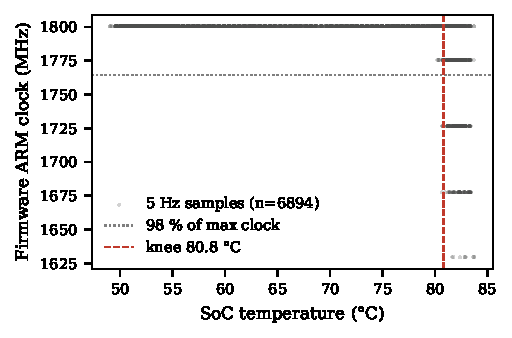
\includegraphics[width=\columnwidth]{figures/fig1_exp1_knee.pdf}
\caption{Experiment~1: firmware ARM clock against SoC temperature (6{,}894 samples at 5\,Hz, four-core load). The
knee (80.8\degC{}) is the lowest temperature at which the clock fell below 98\,\% of its maximum. Points are
jittered by $\pm0.15$\degC{} for visibility.}
\label{fig:knee}
\end{figure}

\subsection{G2: service time against temperature}\label{sec:g2}
In Experiment~2, run~3 (2 ramps, 3{,}027 HOT jobs, 36 kept bins), the OLS slope of bin-median latency on bin-median
temperature is \textbf{+0.208\,ms/\textdegree{}C} (95\,\% cluster-bootstrap CI [+0.070, +0.343]). G2 is
\textbf{PASS}.

The relationship is a step at the knee, not a line (Fig.~\ref{fig:sT}):
\begin{itemize}
\item \textbf{Below the knee:} bin medians stay within 196.23--196.55\,ms in all 30 bins, from 47.7 to 79.4\degC{}.
\item \textbf{Just above it:} 197.4--198.0\,ms at 81.3--81.8\degC{}.
\item \textbf{On the plateau:} 207.9--208.5\,ms at 83.3\degC{} and 211.0--212.1\,ms at 84.2\degC{}.
\end{itemize}

\begin{figure}[t]
\centering
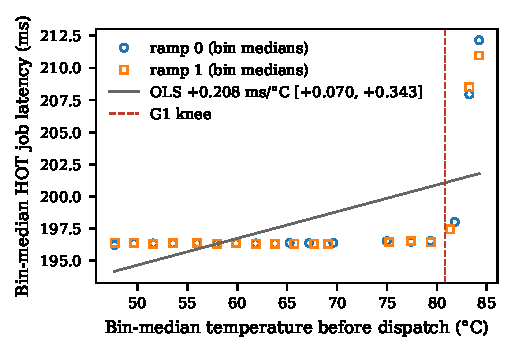
\includegraphics[width=\columnwidth]{figures/fig2_exp2_sT.pdf}
\caption{Experiment~2 (run~3): bin-median HOT job latency against bin-median temperature before dispatch (2\degC{}
bins, $\ge$20 jobs, two ramps). The preregistered OLS slope and its cluster-bootstrap CI summarise a step at the
80.8\degC{} knee.}
\label{fig:sT}
\end{figure}

\subsection{G3: cold-latency match}
In the accepted workload validation (40 pairs), median latency was 196.32\,ms for HOT and 196.22\,ms for COOL. The
gap is $-0.050$\,\% (95\,\% CI [$-0.080$, $-0.001$]\,\%), class TARGET MET. G3 is \textbf{PASS}.

\subsection{Session validity}
The Experiment~3 session ran 40 of 40 scheduled sequences in about 3\,h.
\begin{itemize}
\item All sequences were valid (10 per ordering), with no reruns.
\item No under-voltage was flagged, no watchdog signal was sent, and cleanup was verified.
\item Every sequence had exactly 300 HOT and 300 COOL jobs in its ordering's structure, and all 24{,}000 jobs
completed their planned units.
\end{itemize}
The A7 validity rule is met.

\subsection{G4: ordering and time above the knee}
Ordering changed the thermal trajectory (Fig.~\ref{fig:traj}, Fig.~\ref{fig:tak}, Table~\ref{tab:summary}):
\begin{itemize}
\item \code{hot\_first} ran up toward the knee during its HOT half.
\item \code{cool\_first} first cooled to about 61\degC{}, then climbed.
\item \code{alternating} and \code{random} settled near 71--72\degC{}.
\end{itemize}
Median time above the knee per sequence was 13.3\,s (\code{hot\_first}), 0.8\,s (\code{cool\_first}) and 0\,s
(\code{alternating}, \code{random}). The preregistered contrast between the largest and smallest median is
\textbf{+13.3\,s, 95\,\% CI [+6.0, +23.8]}. G4 is \textbf{PASS}.

\begin{figure}[t]
\centering
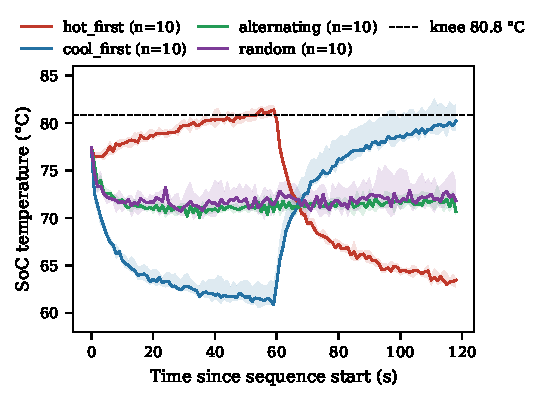
\includegraphics[width=\columnwidth]{figures/fig3_exp3_trajectories.pdf}
\caption{Experiment~3: SoC temperature during the 600-job sequences; median (line) and interquartile range (band)
across the 10 sequences of each ordering, aligned at sequence start.}
\label{fig:traj}
\end{figure}

\begin{figure}[t]
\centering
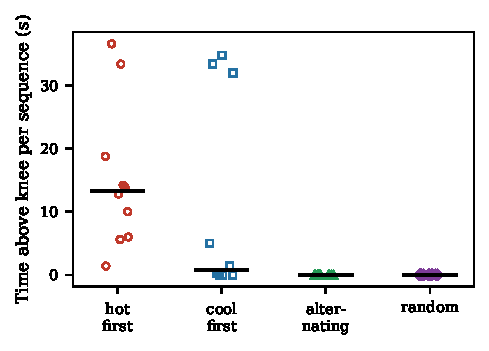
\includegraphics[width=\columnwidth]{figures/fig4_exp3_time_above_knee.pdf}
\caption{Experiment~3: time above the 80.8\degC{} knee per sequence (points) and per-ordering median (bar).}
\label{fig:tak}
\end{figure}

\begin{table*}[t]
\centering
\caption{Per-ordering summary, median [interquartile range] over 10 valid sequences each}
\label{tab:summary}
\footnotesize
\begin{tabular}{@{}lllll@{}}
\toprule
 & hot\_first & cool\_first & alternating & random\\
\midrule
Time above knee (s) & 13.3 [7.0, 17.7] & 0.8 [0.0, 25.3] & 0.0 [0.0, 0.0] & 0.0 [0.0, 0.0]\\
Peak temperature (\textdegree{}C) & 82.3 & 81.1 & 77.4 & 77.4\\
P99 latency (ms) & 201.26 [201.05, 201.61] & 201.35 [200.27, 207.60] & 202.14 [201.76, 202.42] & 201.51 [201.34, 201.83]\\
P95 latency (ms) & 199.39 & 199.44 & 199.40 & 199.34\\
Mean latency (ms) & 197.14 & 197.11 & 197.20 & 197.09\\
Throughput (jobs/s) & 5.014 & 5.015 & 5.013 & 5.015\\
\bottomrule
\end{tabular}
\end{table*}

\subsection{G5 and G5b: tail latency, mean latency, throughput}
Median per-sequence P99 differed by at most 0.88\,ms (0.44\,\%) between any two orderings (Fig.~\ref{fig:out},
Table~\ref{tab:pairs}).
\begin{itemize}
\item \textbf{Uncorrected:} one pair's CI excluded zero (\code{alternating} $-$ \code{random}, +0.62\,ms,
$p=0.046$).
\item \textbf{Holm:} with six pairs, Holm's first step needs $p\le0.0083$, so no pair survives. G5 is
\textbf{FAIL}.
\item \textbf{Secondary metrics:} for mean latency and throughput, the smallest $p$-values (0.037 and 0.045, the same
pair) also fail Holm's first step. G5b is \textbf{FAIL}.
\end{itemize}

\begin{figure*}[t]
\centering
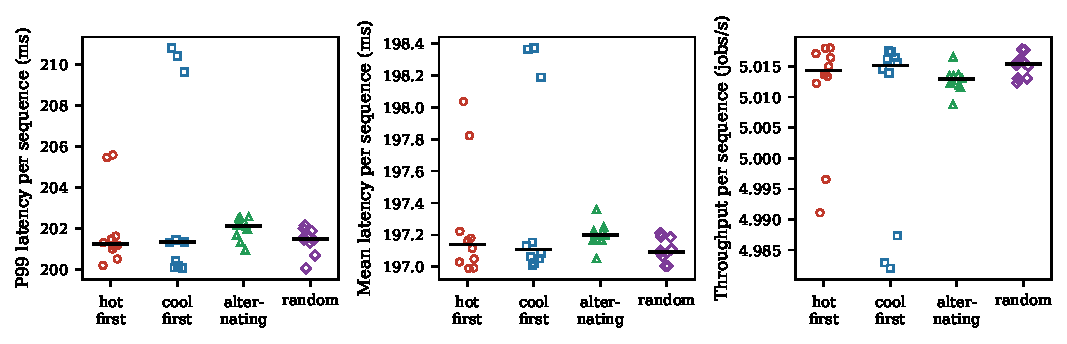
\includegraphics[width=\textwidth]{figures/fig5_exp3_outcomes.pdf}
\caption{Experiment~3: per-sequence P99 latency, mean latency and throughput by ordering (points; horizontal jitter
only), with medians (bars).}
\label{fig:out}
\end{figure*}

\begin{table}[t]
\centering
\caption{Pairwise differences in median per-sequence P99 (ms): bootstrap 95\,\% CI, two-sided bootstrap $p$, Holm
decision, Cliff's $\delta$}
\label{tab:pairs}
\footnotesize
\setlength{\tabcolsep}{3pt}
\begin{tabular}{@{}lrrrcr@{}}
\toprule
Pair & $\Delta$ & 95\,\% CI & $p$ & Holm & $\delta$\\
\midrule
alt $-$ cool & +0.79 & [$-7.66$, +1.97] & 0.306 & no & +0.30\\
alt $-$ hot & +0.88 & [$-1.29$, +1.36] & 0.068 & no & +0.44\\
alt $-$ rand & +0.62 & [+0.01, +1.08] & 0.046 & no & +0.56\\
cool $-$ hot & +0.09 & [$-1.97$, +8.45] & 0.979 & no & +0.00\\
cool $-$ rand & $-0.16$ & [$-1.39$, +8.18] & 0.389 & no & $-0.12$\\
hot $-$ rand & $-0.26$ & [$-0.75$, +1.90] & 0.340 & no & $-0.14$\\
\bottomrule
\end{tabular}
\end{table}

\subsection{G6 and verdict}
G6 is defined only if G4 and G5 both pass. Because G5 failed, G6 is \textbf{not testable}.

The committed analysis code, applied to the Experiment~1--3 records, returns G1--G4 PASS, G5 and G5b FAIL, and the
preregistered verdict \textbf{LIKELY KILL}: the thermal trajectory moves, but no performance metric responds.
Independently written code reproduces this verdict from the raw records.

\subsection{A thermal effect without a performance effect}\label{sec:discussion}
Ordering changed \emph{when} and \emph{for how long} the die was above its knee (G4). It did not move the latency
distribution enough to register in P99, mean latency or throughput (G5, G5b). The exploratory analyses below,
which cannot change the verdict, suggest why.

\textbf{At a two-minute horizon starting just below the knee, throttling is shallow.}
\begin{itemize}
\item Of 12{,}000 HOT jobs, 1{,}258 started at or above the knee. Their median latency was 198.29\,ms, against
196.87\,ms for HOT jobs below it (+0.7\,\%). Their 90th percentiles were 204.99 and 198.98\,ms.
\item The deeper clock reductions behind the 208--212\,ms plateau of Experiment~2 appear only after minutes of
continuous load. A \code{hot\_first} sequence runs at most 60\,s of HOT work.
\item In \code{hot\_first} sequences, a median 60 jobs per sequence (10\,\%) started at or above the knee, but most
of them were only slightly slower.
\end{itemize}

\subsection{What P99 measures for 600 jobs}\label{sec:p99}
Per sequence, P99 is in effect the 7th-largest of 600 latencies, and slow jobs are scarce:
\begin{itemize}
\item The median number of jobs slower than 205\,ms per sequence was 2.5, 2.5, 2.0 and 2.5 across orderings. The
number slower than 200\,ms was 14.5--18.
\item The 7th-largest latency is therefore usually an ordinary job of about 200--202\,ms, not a throttled one, in
every ordering.
\item The rare extreme outliers (11--15 jobs above 215\,ms per ordering, out of 6{,}000) mostly started below the
knee.
\item A job-level bootstrap within a sequence (assuming exchangeable jobs) gives a median 95\,\% interval width of
3.3\,ms for one sequence's P99.
\end{itemize}

\textbf{Sensitivity.} A rough normal approximation on the per-sequence P99 spread suggests that, with 10 sequences
per ordering and 80\,\% power at Holm's first step, detectable effects range from about 0.9\,ms
(\code{alternating} vs \code{random}) to 5.6\,ms (pairs involving \code{cool\_first}). The observed median
differences, $\le0.9$\,ms, are below most of these. A non-significant result is not equivalence. What the data
support is narrower: at this operating point, any ordering effect on the median per-sequence P99 is small relative
to a 196\,ms job, and the observed differences were under 0.5\,\%.

\subsection{Starting state and the session}
The preregistered design fixed a near-knee start (77\degC{}) and a two-minute horizon. Exploratory observations
show how much the outcome depends on thermal state (Fig.~\ref{fig:session}).

\textbf{Repetitions 0--2 (the first $\sim$70\,min):}
\begin{itemize}
\item Median cooldowns to 48.3\degC{} were 152, 217 and 262\,s, and median pre-heats 32--36\,s.
\item In 5 of the 6 \code{hot\_first} and \code{cool\_first} sequences, the die spent 32--37\,s above the knee, and
P99 was 205.5--210.8\,ms.
\item The \code{alternating} and \code{random} sequences of the same repetitions stayed at 200.1--202.6\,ms.
\end{itemize}

\textbf{Repetitions 3--9:} median cooldowns were 57--75\,s and median pre-heats 43--48\,s. P99 was
200.1--202.5\,ms in every ordering.

The cause is unknown; ambient temperature and airflow were not measured. Because every repetition contains all four
orderings, the shift adds variance rather than bias to the ordering comparison, and it produces the wide CIs for the
\code{cool\_first} pairs.

\textbf{A hypothesis, not a result.} When the device is loaded enough that blocked orderings spend more than about
30\,s above the knee within a sequence, ordering may move P99 by several milliseconds (2--5\,\%). That would need a
separately preregistered study with controlled ambient conditions.

\textbf{Pooling.} Pooling all 6{,}000 jobs of an ordering gives P99 values of 204.1, 207.9, 202.2 and 201.6\,ms
(Fig.~\ref{fig:ccdf}). These are dominated by the few hot early sequences. They are not the preregistered
statistic, but they show that the choice of summary changes the impression.

\begin{figure}[t]
\centering
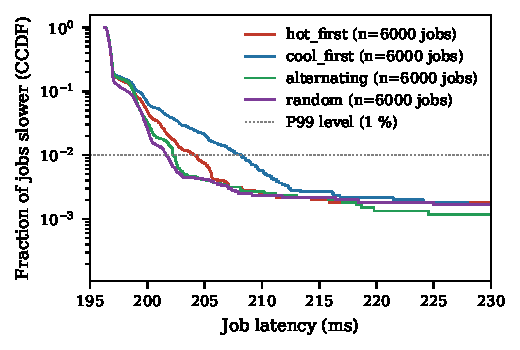
\includegraphics[width=\columnwidth]{figures/fig6_exp3_tail_ccdf_exploratory.pdf}
\caption{Exploratory: complementary CDF of job latency, all 6{,}000 jobs of each ordering (log scale). Not the
preregistered statistic; pooled tails are dominated by a few early-session sequences.}
\label{fig:ccdf}
\end{figure}

\begin{figure}[t]
\centering
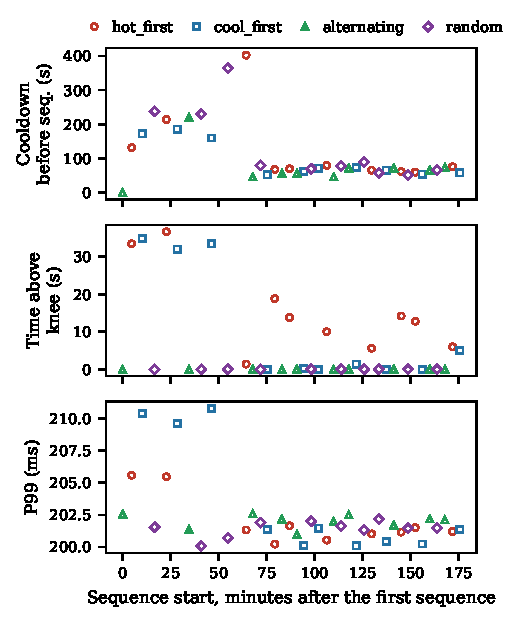
\includegraphics[width=\columnwidth]{figures/fig7_exp3_session_order_exploratory.pdf}
\caption{Exploratory: cooldown before each sequence, time above the knee, and P99 per sequence against session time.
The first $\sim$70\,min show long cooldowns and, for the blocked orderings, long times above the knee and higher
P99. (The first sequence needed no cooldown.)}
\label{fig:session}
\end{figure}

\subsection{Alternative explanations and supported claims}\label{sec:claims}
\textbf{Order effects.} Job-length differences are excluded within the validated tolerance (G3). Linear drift is
balanced by the schedule. Nonlinear drift is not excluded, but it is symmetric across orderings within each
repetition.

\textbf{Non-thermal outliers.} The extreme outliers above 215\,ms were spread evenly across orderings and mostly
started below the knee. This suggests operating-system or timing noise rather than throttling.

\textbf{Measurement perturbation.} The between-job flag reads and the 60\,s status observer were present in all
orderings alike.

\textbf{What we can and cannot conclude.}
\begin{itemize}
\item \textbf{Supported:} the causal claim that ordering changes time above the knee. The orderings were randomised
in order and the work was identical.
\item \textbf{Not supported:} the claim that ordering has \emph{no} effect on tail latency. The data allow small
effects, and larger ones in thermal states the session did not control.
\item \textbf{Physical versus practical:} the physical effect (G4) is real. A practically useful effect was not
observed.
\end{itemize}

\subsection{Limitations and threats to validity}\label{sec:limits}
\textbf{Generalisability.}
\begin{itemize}
\item One device and one environment; the bare-board configuration was confirmed afterwards, not logged on the day.
\item Ambient temperature was not measured.
\item One synthetic GEMM workload, without the memory, I/O or accelerator behaviour of real inference.
\item One sequence length (600 jobs) and one start band (77\degC{}); the protocol's sweep of three start
temperatures was not run.
\end{itemize}

\textbf{Power and percentile estimation.} Ten sequences per ordering cannot resolve sub-millisecond P99 effects.
P99 over 600 jobs rests on about 7 order statistics.

\textbf{Statistical assumptions.}
\begin{itemize}
\item The bootstrap assumes exchangeable sequences despite serial execution and a mid-session shift.
\item G4 compares a pair selected from the data, as preregistered.
\item Holm controls error within each metric only.
\end{itemize}

\textbf{Sensors.} The sensor is quantised at 0.487\degC{} and sampled at 5\,Hz. Time above the knee uses sysfs
temperature, not the firmware clock.

\textbf{Interference.} Between-job flag reads use a short-lived process, and a status observer polled every
60\,s. Both were present in all orderings.

\textbf{Process.} One amendment (A5) was approved under delegation before the experimenter reviewed it. Two Experiment~2
runs were inconclusive before G2 was decided. Both are disclosed.

\section{Conclusion and Future Scope}
On a passively cooled Raspberry Pi~4 running matched fixed-work four-core jobs, the order of an identical job
multiset changed how long the device spent above its throttling knee. At the preregistered operating point
(600-job sequences starting at 77\degC{}), that change did not produce a statistically supported difference in P99
latency, mean latency or throughput. The preregistered verdict is LIKELY KILL for the claim that ordering alone
improves tail latency on this device.

\textbf{Future scope.} The following are future experiments, not findings. Each needs its own preregistered
hypothesis, protocol and success criteria, and none can revise this verdict:
\begin{itemize}
\item longer hot blocks that reach the deep throttling plateau, within safety limits;
\item controlled initial thermal states and ambient conditions;
\item tail-sensitive designs sized by a power analysis from the variance reported here;
\item other devices, cooling configurations and real inference workloads.
\end{itemize}

\ifdefined\REVIEW\else
\section*{Author Contributions}
Srijan Srivastava carried out the research and prepared the paper. Padma Priya supervised the work and provided guidance.
\fi

\section*{Acknowledgment}
The authors used Claude (Anthropic), a generative AI assistant, throughout this work to help write and test the code, analyse the data, and draft the text and figures, and it approved amendment A5 under delegation; the authors reviewed the output and take full responsibility for the content.

\begin{thebibliography}{18}
\bibitem{brooks2001} D.~Brooks and M.~Martonosi, ``Dynamic thermal management for high-performance microprocessors,'' in \emph{Proc. 7th Int. Symp. High-Performance Computer Architecture (HPCA)}, 2001, pp. 171--182, doi: 10.1109/HPCA.2001.903261.
\bibitem{skadron2003} K.~Skadron, M.~R. Stan, W.~Huang, S.~Velusamy, K.~Sankaranarayanan, and D.~Tarjan, ``Temperature-aware microarchitecture,'' in \emph{Proc. 30th Annu. Int. Symp. Computer Architecture (ISCA)}, 2003, pp. 2--13, doi: 10.1145/859618.859620.
\bibitem{choi2007} J.~Choi, C.-Y. Cher, H.~Franke, H.~Hamann, A.~Weger, and P.~Bose, ``Thermal-aware task scheduling at the system software level,'' in \emph{Proc. Int. Symp. Low Power Electronics and Design (ISLPED)}, 2007, pp. 213--218, doi: 10.1145/1283780.1283826.
\bibitem{yang2008} J.~Yang, X.~Zhou, M.~Chrobak, Y.~Zhang, and L.~Jin, ``Dynamic thermal management through task scheduling,'' in \emph{Proc. IEEE Int. Symp. Performance Analysis of Systems and Software (ISPASS)}, 2008, pp. 191--201, doi: 10.1109/ISPASS.2008.4510751.
\bibitem{chrobak2008} M.~Chrobak, C.~D\"urr, M.~Hurand, and J.~Robert, ``Algorithms for temperature-aware task scheduling in microprocessor systems,'' in \emph{Algorithmic Aspects in Information and Management (AAIM)}, ser. Lecture Notes in Computer Science.\hskip 1em plus 0.5em minus 0.4em\relax Springer, 2008, pp. 120--130, doi: 10.1007/978-3-540-68880-8\_13.
\bibitem{coskun2008} A.~K. Coskun, T.~S. Rosing, K.~A. Whisnant, and K.~C. Gross, ``Static and dynamic temperature-aware scheduling for multiprocessor SoCs,'' \emph{IEEE Trans. Very Large Scale Integr. (VLSI) Syst.}, vol.~16, no.~9, pp. 1127--1140, 2008, doi: 10.1109/TVLSI.2008.2000726.
\bibitem{sahin2016} O.~Sahin and A.~K. Coskun, ``Providing sustainable performance in thermally constrained mobile devices,'' in \emph{Proc. 14th ACM/IEEE Symp. Embedded Systems for Real-Time Multimedia (ESTIMedia)}, 2016, pp. 72--77, doi: 10.1145/2993452.2994309.
\bibitem{rpi-thermal} Raspberry Pi Ltd, ``Raspberry Pi computer hardware: Frequency management and thermal control,'' Raspberry Pi Documentation. [Online]. Available: \url{https://www.raspberrypi.com/documentation/computers/raspberry-pi.html} (accessed Oct. 18, 2026).
\bibitem{rpi-throttled} Raspberry Pi Ltd, ``Raspberry Pi OS: vcgencmd get\_throttled,'' Raspberry Pi Documentation. [Online]. Available: \url{https://www.raspberrypi.com/documentation/computers/os.html} (accessed Oct. 18, 2026).
\bibitem{dean2013} J.~Dean and L.~A. Barroso, ``The tail at scale,'' \emph{Commun. ACM}, vol.~56, no.~2, pp. 74--80, 2013, doi: 10.1145/2408776.2408794.
\bibitem{zhang2016} Y.~Zhang, D.~Meisner, J.~Mars, and L.~Tang, ``Treadmill: Attributing the source of tail latency through precise load testing and statistical inference,'' in \emph{Proc. ACM/IEEE 43rd Annu. Int. Symp. Computer Architecture (ISCA)}, 2016, pp. 456--468, doi: 10.1109/ISCA.2016.47.
\bibitem{hyndman1996} R.~J. Hyndman and Y.~Fan, ``Sample quantiles in statistical packages,'' \emph{Amer. Statistician}, vol.~50, no.~4, pp. 361--365, 1996, doi: 10.1080/00031305.1996.10473566.
\bibitem{efron1979} B.~Efron, ``Bootstrap methods: Another look at the jackknife,'' \emph{Ann. Statist.}, vol.~7, no.~1, pp. 1--26, 1979, doi: 10.1214/aos/1176344552.
\bibitem{holm1979} S.~Holm, ``A simple sequentially rejective multiple test procedure,'' \emph{Scand. J. Statist.}, vol.~6, pp. 65--70, 1979. [Online]. Available: \url{https://www.jstor.org/stable/4615733}
\bibitem{cliff1993} N.~Cliff, ``Dominance statistics: Ordinal analyses to answer ordinal questions,'' \emph{Psychol. Bull.}, vol.~114, no.~3, pp. 494--509, 1993, doi: 10.1037/0033-2909.114.3.494.
\bibitem{hoefler2015} T.~Hoefler and R.~Belli, ``Scientific benchmarking of parallel computing systems: Twelve ways to tell the masses when reporting performance results,'' in \emph{Proc. Int. Conf. High Performance Computing, Networking, Storage and Analysis (SC)}, 2015, pp. 1--12, doi: 10.1145/2807591.2807644.
\bibitem{mytkowicz2009} T.~Mytkowicz, A.~Diwan, M.~Hauswirth, and P.~F. Sweeney, ``Producing wrong data without doing anything obviously wrong!'' in \emph{Proc. 14th Int. Conf. Architectural Support for Programming Languages and Operating Systems (ASPLOS)}, 2009, pp. 265--276, doi: 10.1145/1508244.1508275.
\bibitem{nosek2018} B.~A. Nosek, C.~R. Ebersole, A.~C. DeHaven, and D.~T. Mellor, ``The preregistration revolution,'' \emph{Proc. Natl. Acad. Sci. USA}, vol.~115, no.~11, pp. 2600--2606, 2018, doi: 10.1073/pnas.1708274114.
\end{thebibliography}

\end{document}
